\chapter{Evoluindo uma plataforma de rede social}
\label{evol-rede-social}

Neste capítulo é discutida a plataforma Noosfero, desde sua arquitetura até os processos de desenvolvimento da comunidade. Além disso, é apresentado o Comunidade.UnB, rede de colaboração livre, no qual são propostas evoluções para que se torne um ambiente híbrido utilizado por professores e alunos.

\section{Noosfero}
\label{noosfero}

O Noosfero \footnote{Disponível em: \url{http://www.noosfero.org}} é uma plataforma livre para criação de redes sociais, desenvolvida em 2007, pela Cooperativa de Tecnologias Livres - Colivre \footnote{Disponível em: \url{http://www.colivre.coop.br}}, sob a licença AGPL\footnote{Licença de software GNU} V3, com a proposta de facilitar a criação de redes sociais personalizadas, livres e autônomas e a geração de conteúdo colaborativo.

Além das funcionalidades de rede social, com foco na produção e compartilhamento de conteúdo, o Noosfero permite que dentro da rede cada usuário e comunidade tenha o seu espaço com total flexibilidade de personalização visual e gerenciamento de conteúdo. São exemplos de portais que utilizam o Noosfero: o Participa BR \footnote{Disponível em: \url{https://www.participa.br/}}, Stoa\footnote{Disponível em: \url{http://stoa.usp.br/}}, Portal da FGA\footnote{Disponível em: \url{http://fga.unb.br/}} e o novo Portal do Software público Brasileiro \footnote{Disponível em: \url{https://portal.softwarepublico.gov.br/}}.

O Noosfero foi desenvolvido na linguagem de programação Ruby, atualmente na versão 2.2.0, e utiliza o \textit{framework} aplicações web \textit{Ruby on Rails} \footnote{Disponível em: \url{http://rubyonrails.org/}}, versão 3.2.21. E utiliza também padrões arquiteturais de software Model-View-Controller (MVC), e o padrão de plugins que serão apresentados na seção \ref{arquitetura}.

A escolha da linguagem \textit{Ruby} foi decisiva no Noosfero, pois possui uma sintaxe simples, que facilita a manutenibilidade do sistema, característica importante em projetos de software livre que tendem a atrair colaboradores externos \cite{meirelles2013}. A escolha do \textit{Rails} foi influenciada pelos seus conceitos básicos que auxiliam em sua produtividade: ``Não Repita a Si Mesmo'' (DRY-\textit{Don't Repeat Yourself}) e ``convenção sobre configuração'' (\textit{Convention Over Configuration}) \cite{akita2006repensando}. Além disso , por questões de segurança, o Noosfero é homologado para a versão \textit{stable} do \textit{Debian}, acompanhando a versão do \textit{Ruby} e do \textit{Rails} dessa distro.

\subsection{Práticas de desenvolvimento da comunidade Noosfero}
\label{proc-desenvol-comunidade}
% - ciclos
% - repositorio
% - commiters/revisao
% - testes

Para que novos desenvolvedores colaborem com o Noosfero, a comunidade utiliza em seu próprio \textit{site} uma seção para o desenvolvimento. Nessa seção, encontram-se os manuais com os passos para instalação do ambiente, descrição dos \textit{plugins} disponíveis, instruções para a personalização da plataforma através de temas além de informações arquiteturais da plataforma. Para realizar o controle de itens a fazer, como a implementação de novas funcionalidades ou correção de bugs é utilizado um \textit{Issue Tracker} do repositório oficial no GitLab \footnote{Disponível em: \url{https://gitlab.com/noosfero/noosfero}}.

Uma vez que o desenvolvedor ou usuário tenha registro no GitLab, é possível utilizar o \textit{Issue Tracker} para cadastrar novas funcionalidades ou \textit{bugs} de maneira simples seguindo os seguintes passos:

\begin{enumerate}
\item preencher o campo título;
\item definir a descrição do item, se existir, é necessário especificar com qual \textit{plugin} o item está relacionado;
\item associar um desenvolvedor responsável pela sua implementação \textit{issue};
\item definir as \textit{labels} da funcionalidade, onde é especificado ao que está relacionado a nova \textit{issue}.
\end{enumerate}

Após a criação da \textit{issue}, todos os membros da comunidade podem visualizar os dados e especificações, bem como discutir sobre os propósitos e formas de implementação da funcionalidade.

A Figura \ref{issue-tracker} evidencia o \textit{Issue Tracker} do Noosfero onde é possível verificar os itens que foram mapeados e seus respectivos \textit{status}, se ainda estão abertas ou fechadas, além de um filtro para os autores e os marcadores envolvidos à cada uma delas. Dessa forma, é possível priorizar os itens identificados como sendo de maior importância para os usuários e desenvolvedores.

\begin{figure}[h]
    \centering
    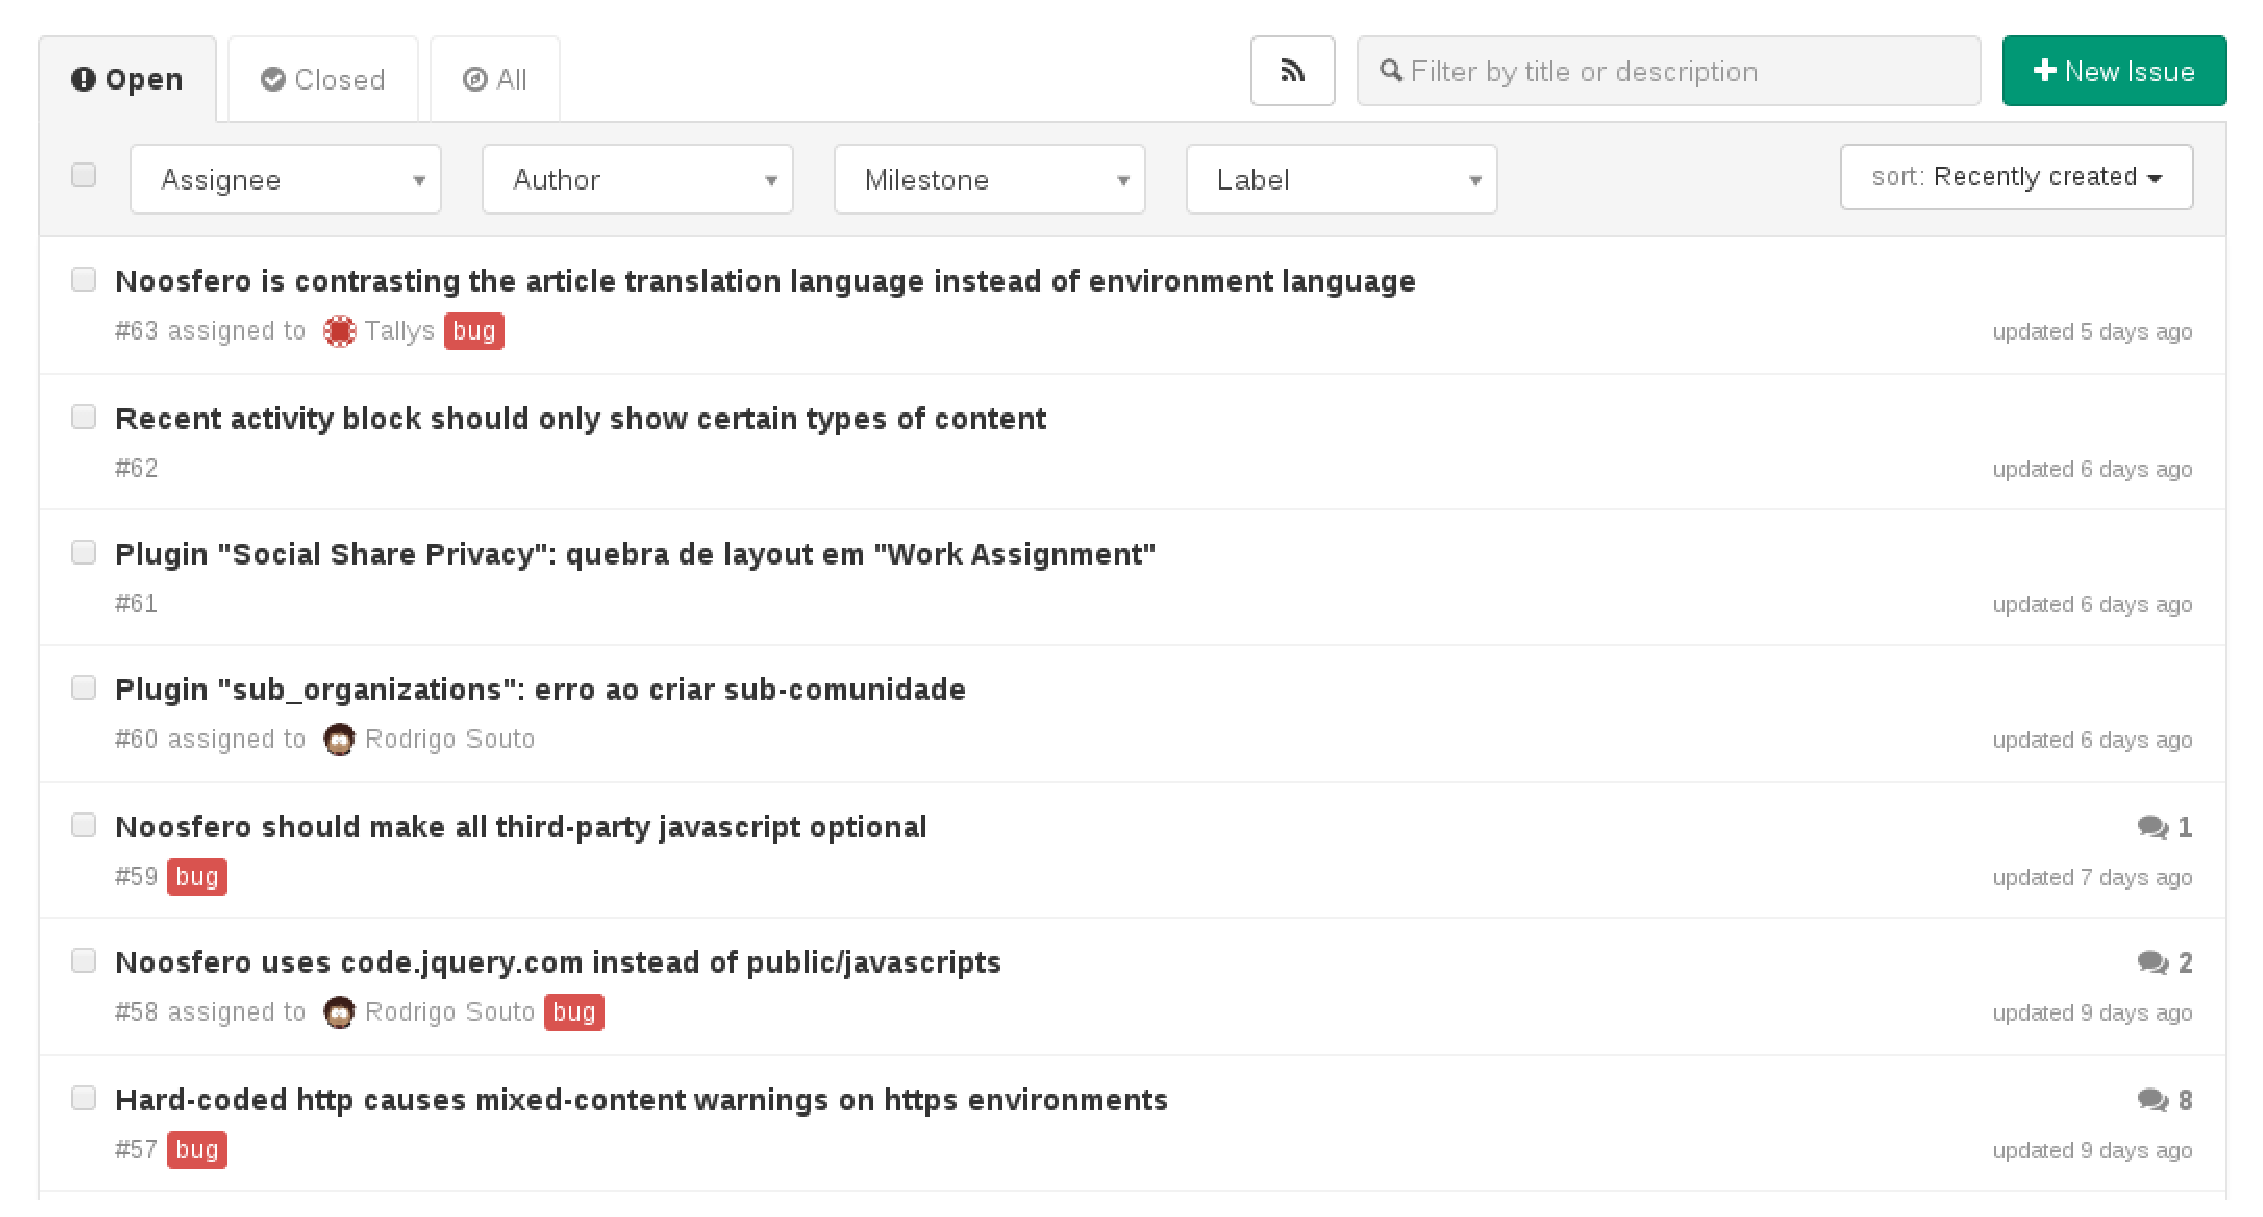
\includegraphics[keepaspectratio=true,scale=0.4]
      {figuras/issueTrackerGitLab.eps}
    \caption{Issue Tracker no GitLab}
    \label{issue-tracker}
\end{figure}

Priorizando a comunicação entre os desenvolvedores, a comunidade compartilha canais \footnote{Canais do Noosfero: \textit{\#noosfero-br} e \textit{\#noosfero}} de comunicação pelo IRC (\textit{Internet Relay Chat}). Nesses os desenvolvedores podem compartilhar conhecimento e realizarem discussões técnicas sobre as implementações.

A implementação é realizada pelo desenvolvedor que tem a responsabilidade de manter a qualidade do código produzido bem como realizar todos os testes relacionados à funcionalidade implementada. Uma vez que este primeiro passo esteja concluído o código é submetido a um \textit{merge-request} onde um dos desenvolvedores do \textit{core} efetua a revisão para verificar se está de acordo com os padrões esperados, e aprova ou não, a inclusão do código na \textit{branch} principal do Noosfero.

A comunidade Noosfero recomenda práticas de desenvolvimento como o TDD, \textit{Test Driven Development} ou Desenvolvimento orientado a testes), combinado com o BDD \footnote{\url{https://cukes.info/}} (\textit{Behavior Driven Development}) ou Desenvolvimento Guiado por Comportamento, que auxiliar o desenvolvedor a criar testes e integrar regras de negócio com a linguagem de programação, mantendo o foco no comportamento do software \cite{north2006introducing}.

Para realizar o controle de versão e gerenciamento do código fonte é utilizado o \textit{Git}, uma ferramenta livre de versionamento distribuído de código fonte. O repositório oficial do Noosfero encontra-se no software livre Gitlab com um espelho no Github\footnote{\url{https://github.com/noosfero/noosfero}}. Na página de desenvolvimento da comunidade existe uma série de recomendações sobre o envio de \textit{patches} para o Noosfero, incluindo como versionamentos e solicitações de inclusão de seu \textit{patch}, ou \textit{merge-request}.

\subsection{Arquitetura}
\label{arquitetura}

Para a evolução de um software de forma adequada é importante o conhecimento da arquitetura do sistema, para não comprometer todo o planejamento realizado na concepção do projeto. Desse modo conhecer e entender a arquitetura de funcionamento do Noosfero é uma etapa fundamental para o densevolvimento de novas funcionalidades para a plataforma.

\begin{figure}[h]
    \centering
    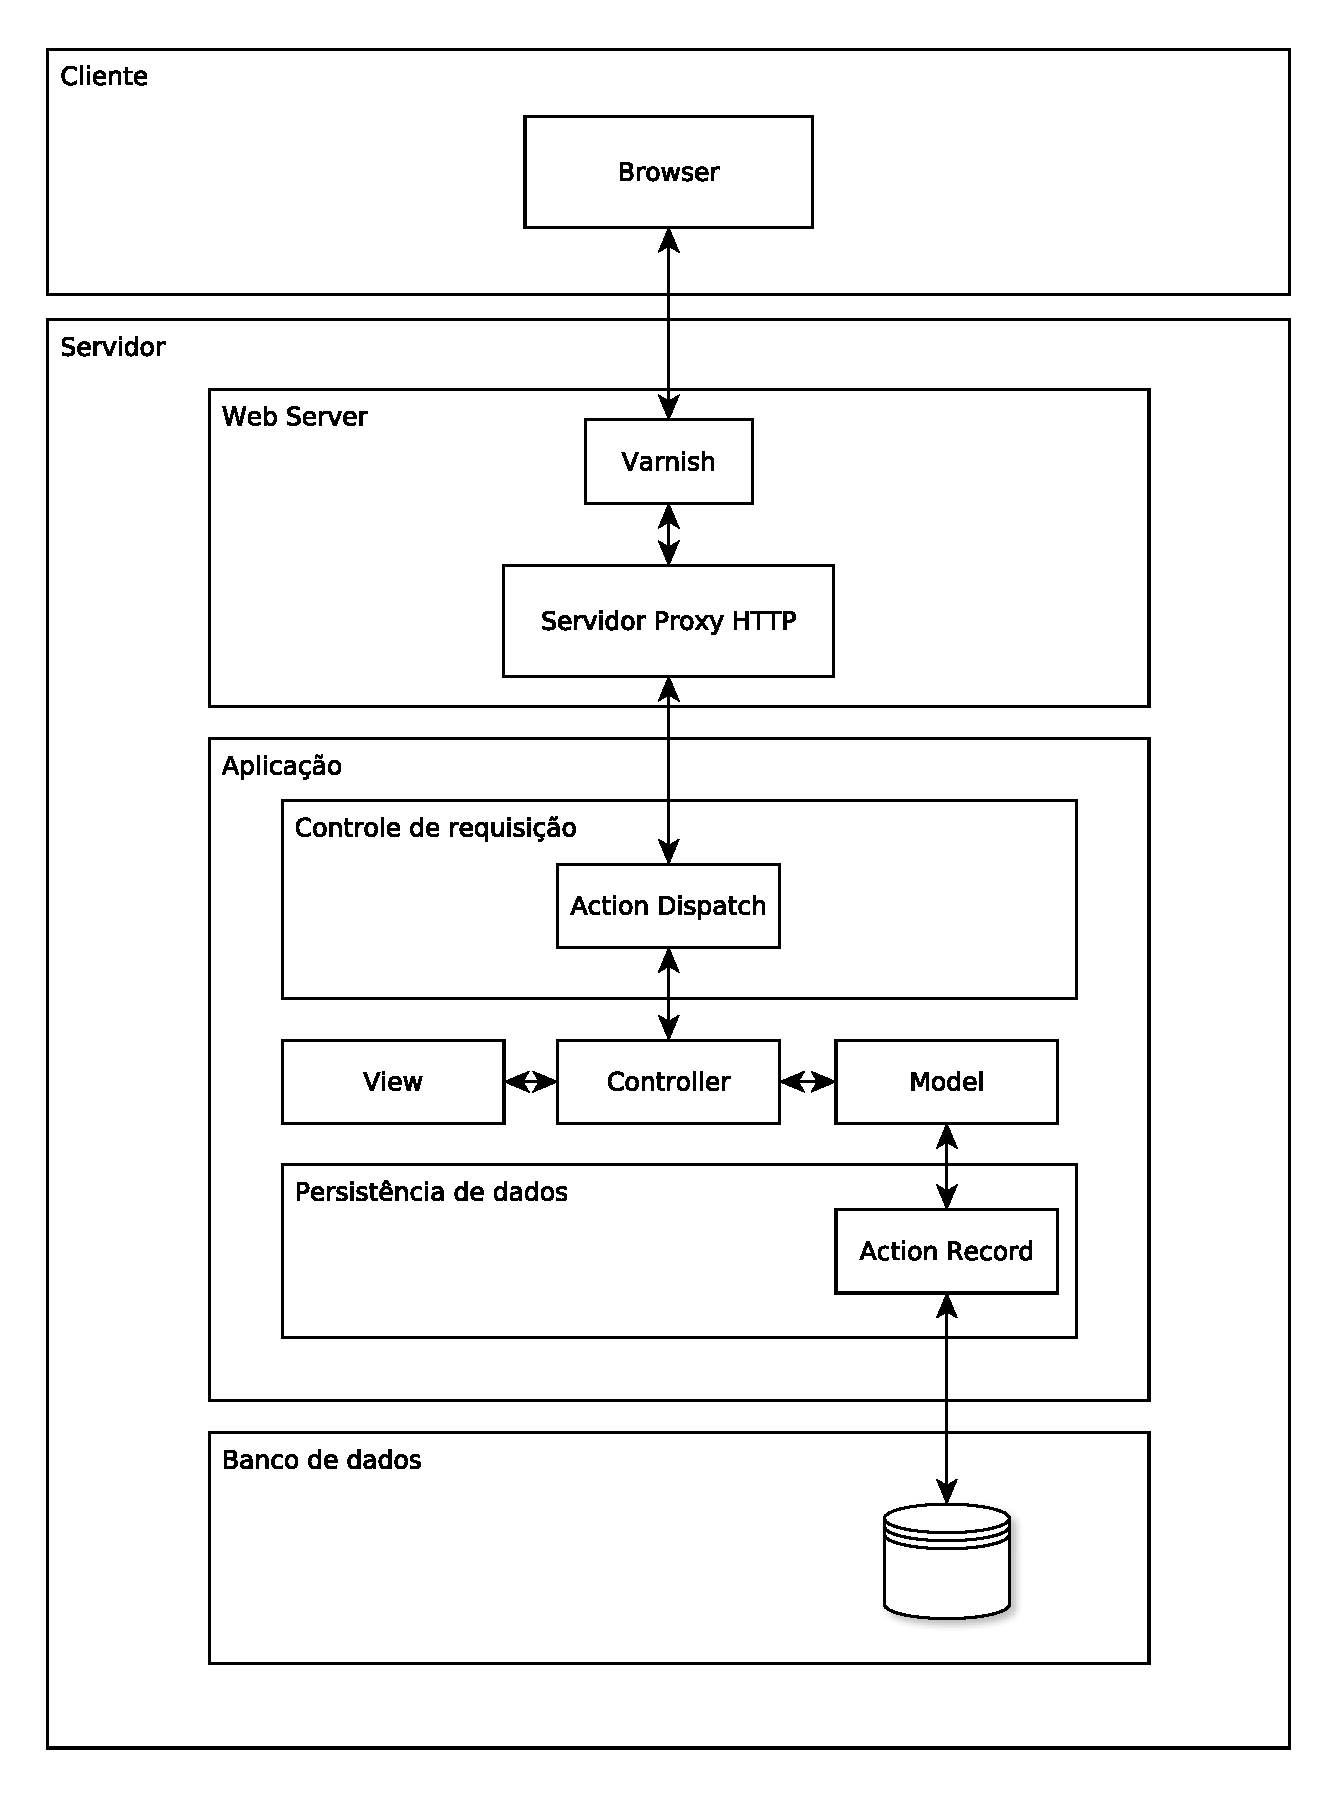
\includegraphics[keepaspectratio=true,scale=0.4]
      {figuras/DiagramaDeArquitetura.eps}
    \caption{Arquitetura do Noosfero}
    \label{arquitetura-noosfero}
\end{figure}

A Figura \ref{arquitetura-noosfero} apresenta uma visão de alto nível da arquitetura do Noofero. Basicamente tem-se uma arquitetura cliente-servidor onde o cliente via \textbf{\textit{Browser}} solicita um conteúdo ou uma função para o servidor Noosfero, que aguarda requisições de entrada para processá-las e compartilhar recursos com o cliente.

Do lado do servidor, temos basicamente três camadas de abstração: \textit{Web-Server}, \textit{aplicação} e \textit{Banco de dados}. Na primeira camada temos dois componentes responsáveis por processar e acelerar todas as requisições de entrada e saída:

\begin{itemize}
\item Varnish: é um acelerador para sites web dinâmicos com alto volume de conteúdo que utiliza \textit{proxy} HTTP Reverso. Sua efiência deve-se ao fato dele armazenar o conteúdo HTTP requisitado na memória RAM, fazendo com que o servidor não consulte e processe diversas vezes o mesmo conteúdo solicitado.
\item Servidor Proxy HTTP: pode ser utilizado o Apache ou Nginx \footnote{\url{http://nginx.org}} que ajudam a melhorar o desempenho funcionando como um servidor proxy HTTP reverso que processa as requisições de entrada e saída e as encaminha para a aplicação executá-las.
\end{itemize}

Na camada da aplicação, foi considerada uma camada responsável pelo controle de requisições, que é efetuada pelo componente \textbf{\textit{Action Dispatch}}, que lida com o mapeamento de todas as requisições, \textit{cookies} e sessão para suas respectivas \textit{controllers}.

Na aplicação, utiliza-se o padrão de arquitetura de software MVC\footnote{Model-view-controller} onde a \textbf{\textit{controller}} controla o fluxo da aplicação,relacionando as entidades de \textit{model} e de \textit{view} através de chamadas de métodos. A \textbf{\textit{model}} representa as entidades do domínio da aplicação, onde a lógica do sistema são implementadas. A \textbf{\textit{view}} é a interface de comunicação com o usuário, ou seja as páginas HTML apresentadas no navegador.

Ainda na camada da aplicação tem-se o \textbf{\textit{Active Record}} que é um ORM \footnote{object-relational mapping}, um mapeador entre objetos e registros de uma tabela, onde cada classe de modelo possui uma tabela correspondente à ela no banco de dados.

Por fim temos a camada de banco de dados que recebe requisições da camada de persistência de dados e por meio de um sistema gerenciador de banco de dados (SGBD) realizam operações na base de dados.

\subsection{Modelo de domínio}

Para \citeonline[p. 160]{larman2002utilizando}, um modelo de domínio é a representação visual de classes conceituais ou objetos do mundo real em um domínio, que também podem ser chamados de modelos conceituais, modelos de objetos de domínio e modelos de objetos de análise. Dessa forma, é necessário o seu entendimento para realizar a evolução da plataforma.

\begin{figure}[h]
    \centering
    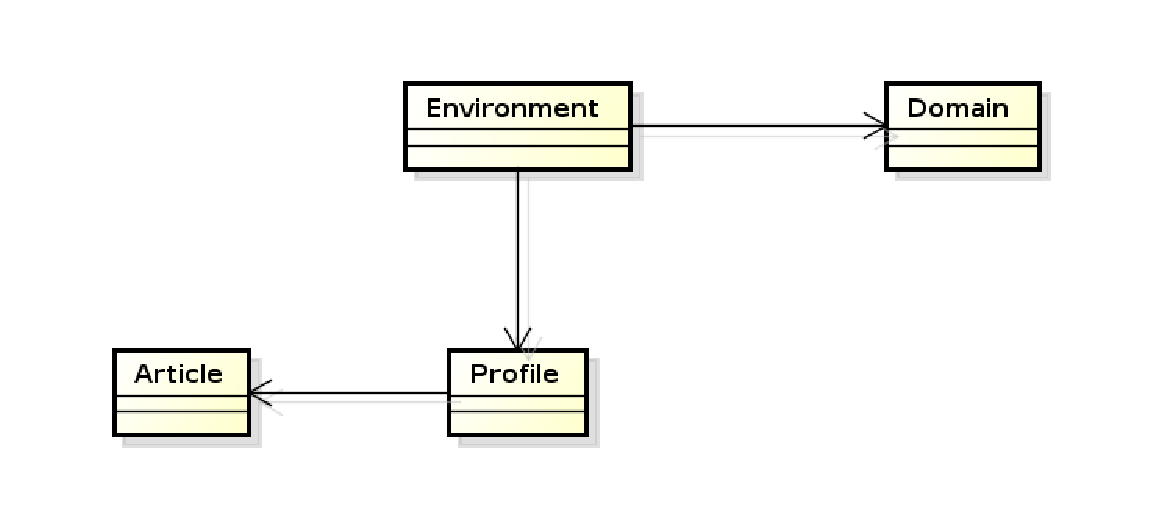
\includegraphics[keepaspectratio=true,scale=0.65]
      {figuras/domain_main.eps}
    \caption{Relações entre entidades de domínio ambiente, domínio e perfis. Extraído de: \cite{bucher2013rede}}
    \label{domain_main}
\end{figure}

O Noosfero é uma plataforma que tem suporte a vários ambientes de rede social dentro de uma mesma instalação. A Figura \ref{domain_main} mostra-se o funcionamento geral do Noosfero com suas quatro principais classes \textbf{\textit{Domain}}, \textbf{\textit{Environment}}, \textbf{\textit{Profile}} e \textbf{\textit{Article}} (Em português: Domínio, Ambiente, Perfil e Artigo respectivamente). Analisando o modelo verifica-se que na implementação é necessário que exista pelo um domínio e partir disso é possível criar várias instâncias de Ambiente na aplicação.

\begin{figure}[h]
    \centering
    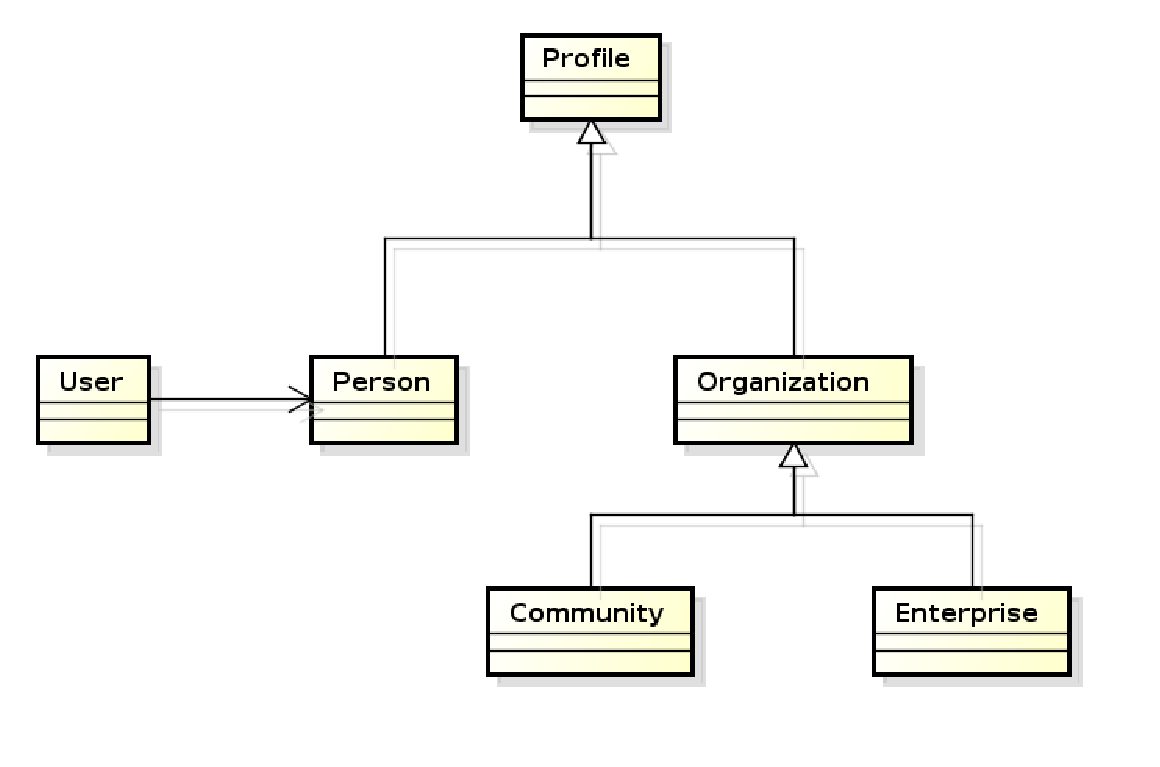
\includegraphics[keepaspectratio=true,scale=0.6]
      {figuras/domain_profiles.eps}
    \caption{Entidades de domínio: tipos de perfis. Extraído de: \cite{bucher2013rede}}
    \label{domain_profiles}
\end{figure}

A entidade Profile é uma generalização das entidades \textbf{\textit{Person}} (Pessoa) e \textbf{\textit{Organization}} (Organização), como pode ser visto na Figura \ref{domain_profiles}. Nesse mesmo modelo percebe-se que Organization é especializada nas entidades concretas \textbf{\textit{Community}} (Comunidade e Enterprise (Empreendimento). A herança é um mecanismo pelo qual qual uma classe sub-classe pode estender uma super-classe, onde basicamente isola-se métodos ou atributos em comum dentro de uma classe pai (super-classe), enquanto as especialidades são responsabilidade das classes filhas (sub-classe).

Por questões de design do código da aplicação foi criada uma entidade \textbf{\textit{User}}, ou Usuário, que é mantida separada da entidade Pessoa, que é quem implementa a lógica de autenticação da aplicação. Desta forma a lógica de autenticação fica separada da lógica de visualização e personalização do perfil.

\begin{figure}[h]
    \centering
    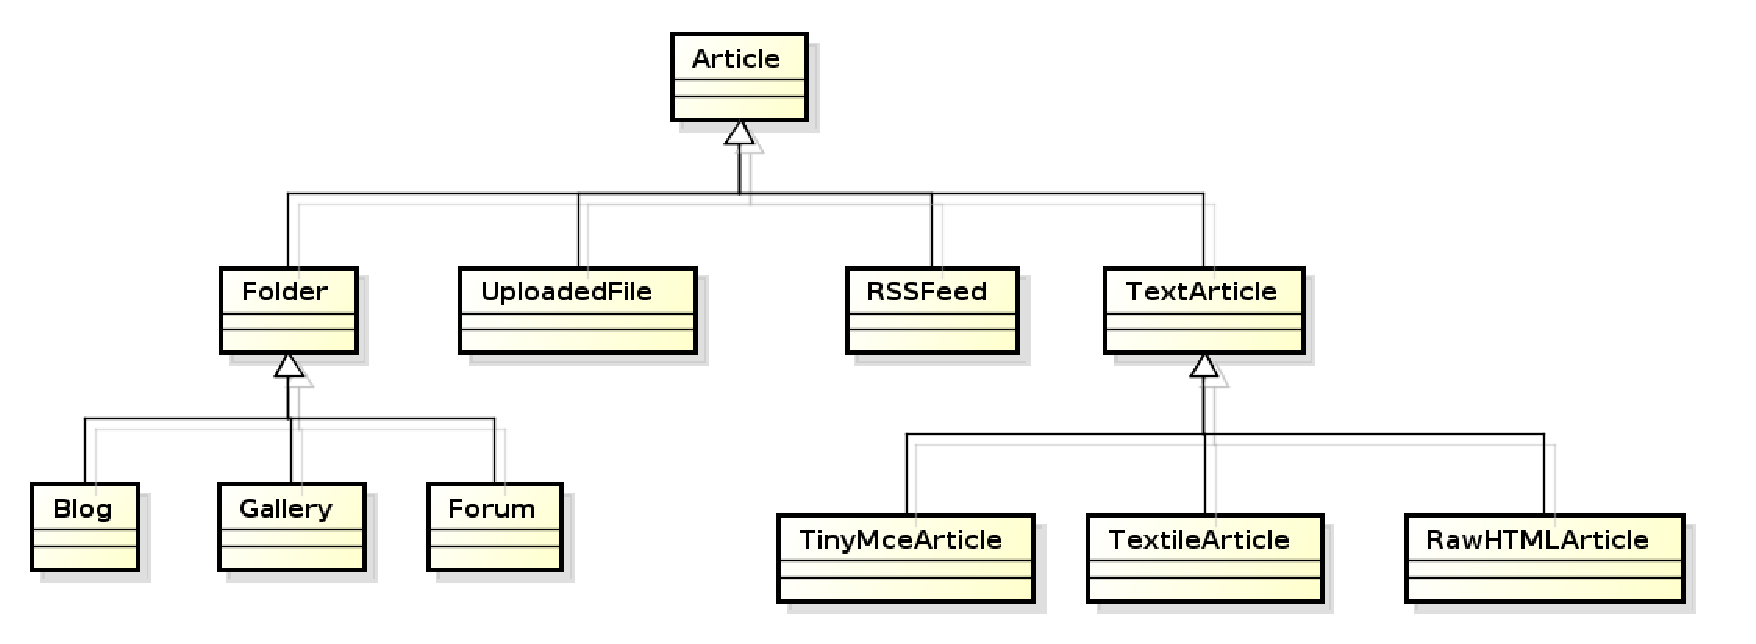
\includegraphics[keepaspectratio=true,scale=0.55]
      {figuras/domain_articles.eps}
    \caption{Entidades de domínio: tipos de artigos. Extraído de: \cite{bucher2013rede}}
    \label{domain_articles}
\end{figure}

Por fim, as entidades mostradas na Figura \ref{domain_articles} representam os principais tipos de conteúdos disponíveis no Noosfero, onde a classe \textbf{\textit{Article}}, ou Artigo, é uma especialização de todos os conteúdos disponíveis como: artigos de texto, pastas, blogs, galerias de imagens, fórum, arquivos e feeds de notícias.

O modelo de domínio aqui apresentado contempla o \textit{core} do noosfero. Para o acréscimo de melhorias e funcionalidades é necessário compreender a visão arquitetural dos \textit{plugins} d a plataforma, que será abordado na próxima seção.

\subsection{Plugins}
\label{plugins-noosfero}

Como é software em constante evolução, a arquitetura do Noosfero foi criada para ser altamente expansível, fazendo-se o uso de \textit{plugins}. Essa arquitetura permite que em cada ambiente fique a critério do usuário quais os \textit{plugins} ou novas funcionalidades serão habilitadas, o que torna o sistema flexível e modular.

% Aumentar figura 6
\begin{figure}[h]
    \centering
    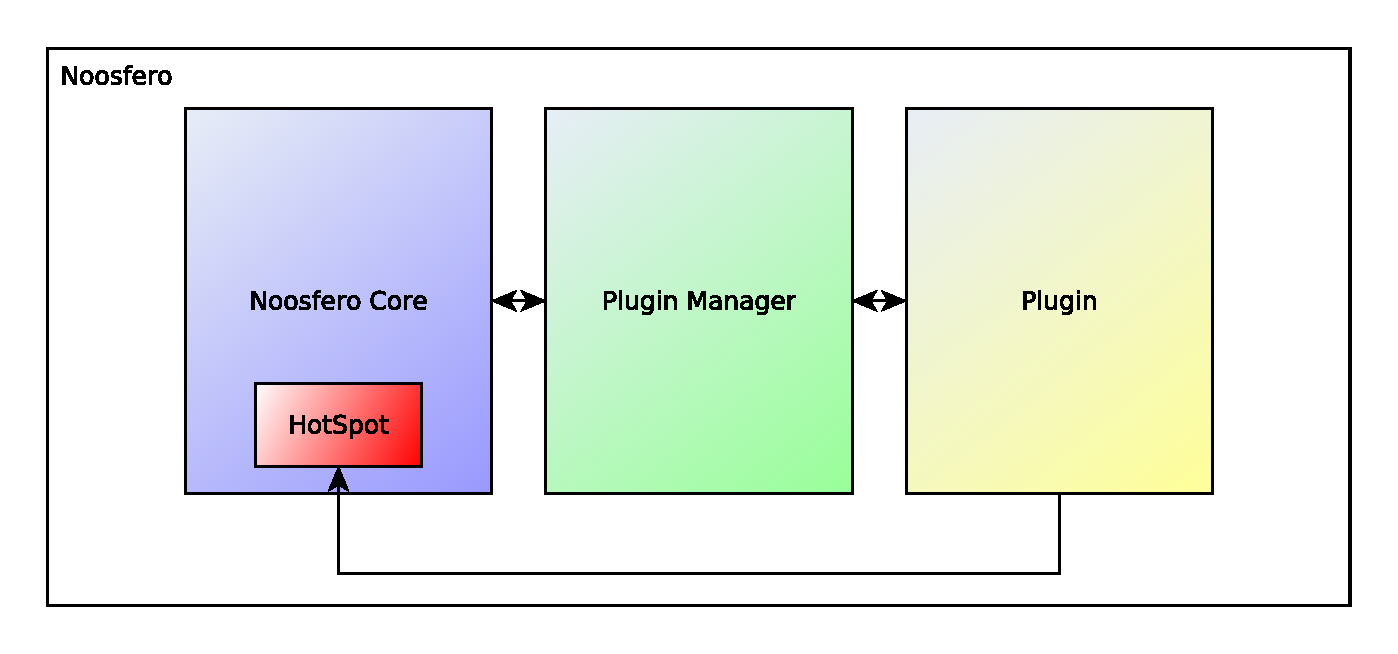
\includegraphics[keepaspectratio=true,scale=0.7]
      {figuras/estruturaDePlugins.eps}
    \caption{Estrutura de Plugins}
    \label{estrutura-plugins}
\end{figure}

A Figura \ref{estrutura-plugins} é uma abstração alto nível do funcionamento interno dos plugins no Noosfero. No \textit{core} do Noosfero temos os \textit{hotspots}, que são pontos de flexibilidade que permitem associar diferentes comportamentos na execução do sistema, permitindo a inserção de trechos de código e ou alteração de um determinado método sem comprometer suas funcionalidades básicas.

Os \textit{hotspots} são gerenciados por uma camada de abstração denominada \textit{Plugin Manager}, ou Gerenciador de \textit{Plugins}, que são chamadas pelo \textit{core} através de um metódo principal conhecido como \textit{dispatch}. Basicamente, o ciclo de execução pode ser descrito da seguinte maneira: durante a execução de alguma funcionalidade o método \textit{dispatch} é invocado por alguma funcionalildade do core, deste modo o gerenciador de plugins verifica todos os \textit{Plugins} que fazem uso daquele \textit{hotspot} e encaminha para cada um deles a execução de suas ações de acordo com sua implementação.

Essa arquitetura extensível adotada pelo Noosfero auxilia no controle da qualidade de código das novas funcionalidades. A camada de \textit{Plugins} localiza-se fora do código do seu núcleo, em uma pasta denominada \textit{plugins} em que desenvolvedor cria novas funcionalidades sem modificar o comportamento \textit{core} do Noosfero, fazendo uso dos \textit{dispatch}.

Adicionalmente como mencionado na Seção \ref{proc-desenvol-comunidade}, o Noosfero faz uso de testes para manter a integridade de seu código, desse modo esta prática é estendida aos \textit{plugins} que devem englobar seus respectivos testes para evitar a inserção de \textit{bugs} e mudanças inesperadas no comportamento do sistema. 

Assim sendo a evolução proposta para este trabalho será realizada através de plugins, como proposto na Seção \ref{desen-noosferAVA}

\section{Comunidade UnB}
\label{comunidade-unb}

A Comunidade.UnB é uma rede colaboração livre desenvolvida para que alunos, professores e servidores técnico-administrativos tenham um ambiente virtual de criação e compartilhamento de conhecimento colaborativo. É um ambiente virtual para o compartilhamento de ideias, produção de conteúdo colaborativo de modo que possam publicá-los para que possa ser de utilidade para outras pessoas ou parcelas da sociedade, uma vez que acredita-se que este é um dos papéis de uma Universidade \cite{bucher2013rede}.

\begin{figure}[!htb]
    \centering
    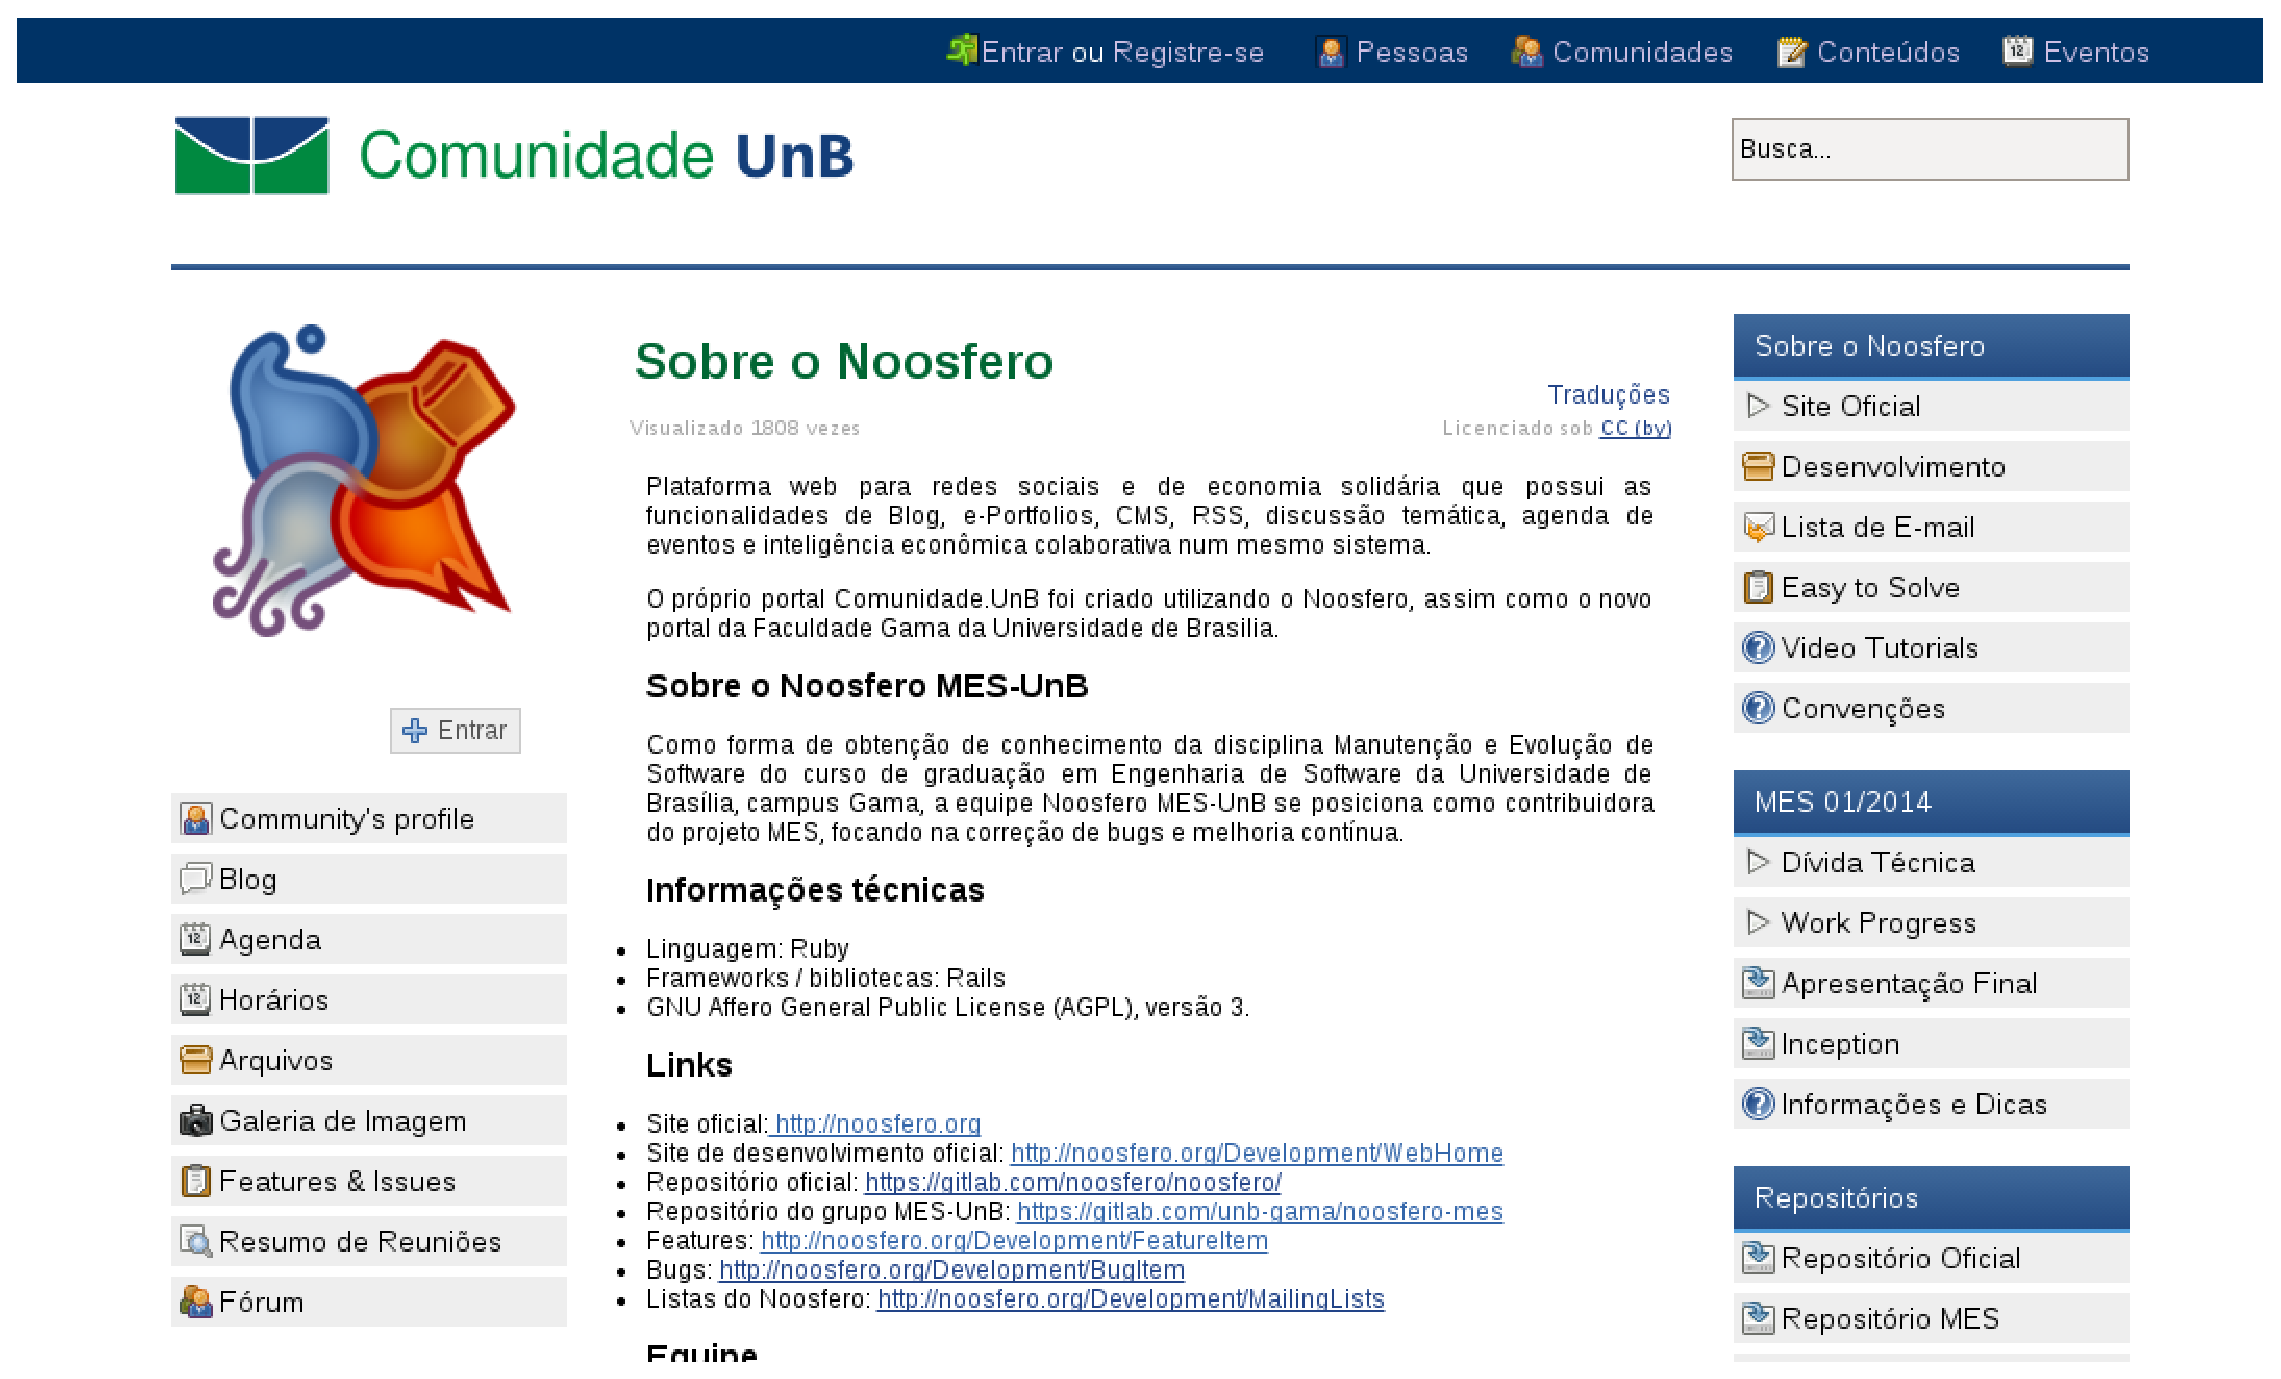
\includegraphics[keepaspectratio=true,scale=0.4]
      {figuras/comunidade-mes.eps}
    \caption{Exemplo do uso do Comunidade.UnB na disciplina de MES.}
    \label{comunidade-mes}
\end{figure}

Inspirada na rede social de colaboração Stoa \footnote{Disponível em: \url{https://social.stoa.usp.br/}}, da Universidade de São Paulo (USP), a Comunidade.UnB foi criada em 2013 a partir de um trabalho de conclusão de curso de Daniel Costa Bucher e até então está disponibilizada em ambiente de testes. Permite ao usuário a criação de seu espaço pessoal e a liberdade de publicar suas ideias, ou o conteúdo que desejar, por exemplo, na forma de blogs pessoais, blogs de disciplinas, pesquisas em andamento, dentre outras, além de compartilhar esse conteúdo para ser acessível para outros usuários dentro e fora da rede.

O Noosfero, descrito na Seção \ref{noosfero}, foi a plataforma utilizada para o desenvolvimento da Comunidade.UnB, por dispor de um grande potencial e devido às suas funcionalidades avançadas, que permitem a criação e o compartilhamento de conteúdo de forma satisfatória. Além de dispor de uma comunidade ativa e de posição geográfica favorável em relação ao seu núcle de desenvolvimento que se encontra no Brasil, facilitando a comunicação com os seus principais desenvolvedores.

Apesar da Comunidade.UnB estar disponibilizada como um ambiente de testes e não possuir uma vasta divulgação pela Universidade de Brasília, no seu primeiro ano de criação contava com 153 usuários e 14 comunidades. Ao final de maio de 2015 contabilizava 376 usuários e 30 comunidades demonstrando que houve crescimento.

Alguns professores adotaram a Comunidade.UnB como um ambiente de apoio ao Moodle, AVA oficial adotado pela UnB. Na Figura \ref{comunidade-mes} é apresentado um exemplo de seu uso na disciplina de Manutenção e Evolução de Software (MES) ministrada pelo professor Paulo Roberto Miranda Meirelles.

Esse é um exemplo de comunidade criada dentro do Comunidade.UnB, que possui características que se assemelham ao ambiente Moodle, como evidenciado na Seção \ref{comparacao-ava}, carece de alguns funcionalidades importantes mas com a vantagem da possibilidade de acesso do público ao conteúdo, e a continuidade do conteúdo desenvolvido por outras pessoas que eventualmente se juntem ao longo do tempo. Vale lembrar que em uma publicação de conteúdo os níveis de privacidade podem ser alterados basicamente entre públicos e privados.

As limitações da plataforma e a proposta de uso da Comunidade.UnB por professores para a criação de disciplinas, estimulam o desenvolvimento de funcionalidades que levem à plataforma Noosfero a assemelhar-se a um ambiente virtual de aprendizagem. Dessa maneira na Seção \ref{desen-noosferAVA} é apresentada a proposta de estudo desse trabalho para desenvolvimento de funcionalidades e minimização das diferenças entre o Noosfero e os ambientes virtuais de aprendizegem.

\chapter{Desenvolvimento do NoosferAVA}
\label{desen-noosferAVA}

Nesta seção apresentaremos as funcionalidades desenvolvidas para contribuir para a adequação do Noosfero a um ambiente virtual de aprendizagem, para exercer a função de apoio aos AVA adotados pela universidade. Serão apresentados os requisitos funcionais levantados para que esta possa suprir as necessidades levantadas.

Além das funcionalidades relatadas, julgou-se necessária a evolução do \textit{plugin Comunidade.UnB}, iniciado por \citeonline{bucher2013rede}, com objetivo de integrar o Noosfero com o serviço de Lightweight Directory Access Protocol (LDAP). Uma base LDAP é utilizada pela UnB para manter os dados de todos os seus alunos e funcionários.

As funcionalidades podem ser visualizadas no Apêndice \ref{apen-historia-usuario} e estão apresentadas utilizando o formato de histórias de usuários (US) \footnote{Em inglês \textit{User Stories}(US)}, de acordo com as práticas ágeis. Além disso, os critérios de aceitação estão expostos no formato de cenários de uso, utilizando BDD.

% ----------------------------------------------------------------
\section{O processo de desenvolvimento}

O desenvolvimento foi realizado no Laboratório de Produção, Pesquisa e Inovação em Software (LAPPIS) da FGA que é um ambiente para  alunos e professores trabalharem de forma colaborativa na produção de software. No laboratório são adotadas práticas ágeis onde vários de seus integrantes colaboram com o Noosfero.

A partir dos requisitos levantados e levando em consideração as práticas ágeis utilizadas no LAPPIS foram realizadas \textit{sprints} com duração de quinze dias. Em cada uma dessas foram desenvolvidas histórias de acordo com a pontuação e demanda de atividades na equipe do Portal, visto que o desenvolvimento foi realizado de maneira colaborativa.

\begin{figure}[h]
    \centering
    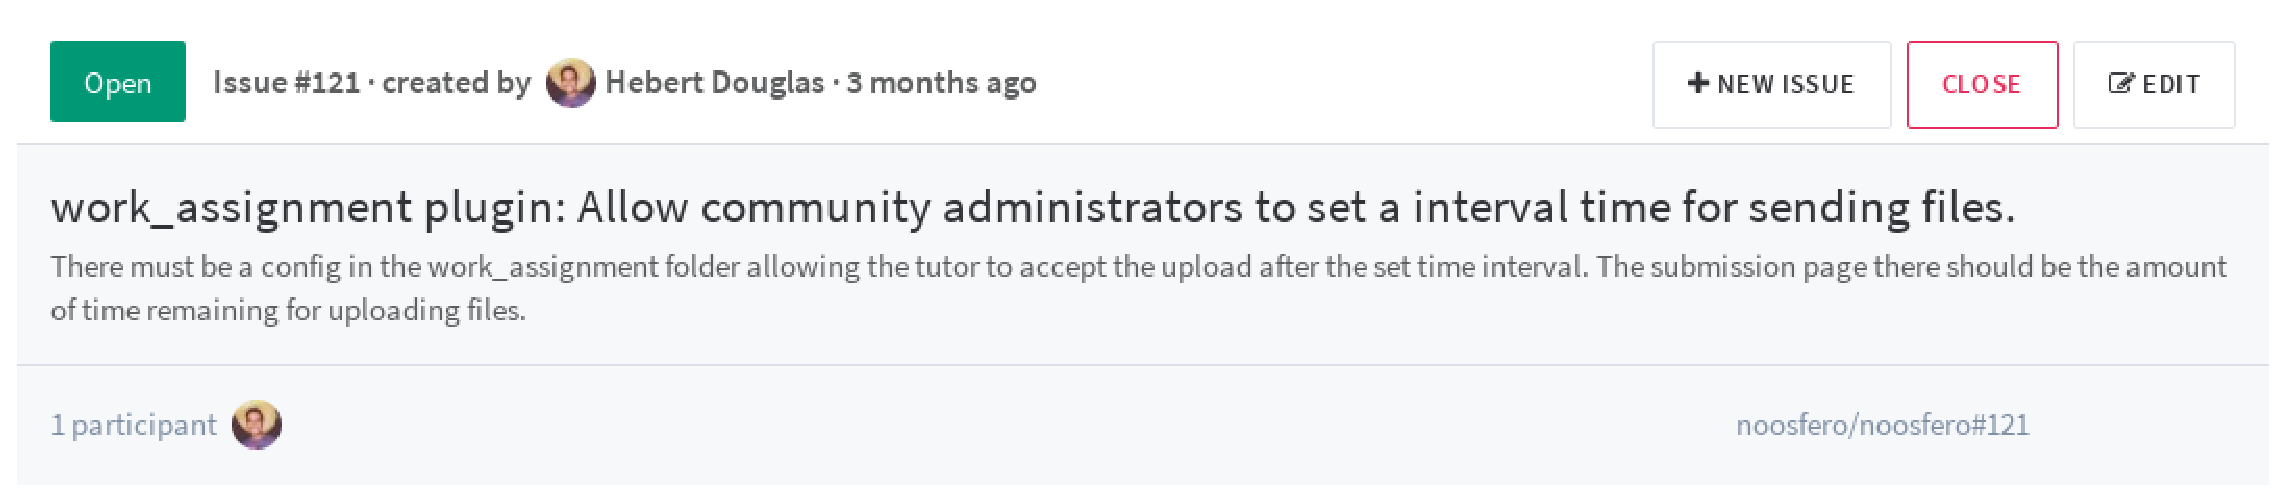
\includegraphics[keepaspectratio=true,scale=0.4]
      {figuras/issue121.eps}
    \caption{Issue 121: Gerenciamento de tempo para work\_assignment}
    \label{fig:issue-121}
\end{figure}

A primeira \textit{sprint} de desenvolvimento das histórias de usuário, foi iniciada em Julho junto com a equipe do Portal FGA. Seguindo as práticas de desenvolvimento da comunidade Noosfero, criou-se uma \textit{Issue} para evidenciar aos desenvolvedores o ínicio da implementação de uma nova funcionalidade. A \textit{Issue} criada foi a de número 121\footnote{Disponível em: \url{https://gitlab.com/noosfero/noosfero/issues/121}} que  é evidenciada na Figura \ref{fig:issue-121}.

Nessa sprint foi desenvolvida a história de usuário (\ref{us01}) ``Definir tempo restante'', que permite ao administrador definir e modificar um tempo limite para envio dos trabalhos no \textit{plugin work assignment}.

Na segunda sprint, foi densenvolvido o último cenário de uso da \ref{us01} que até então não haviam sido resolvidos, ``Permitir entrega de atividades após período''. Este cenário permite ao professor autorizar os alunos a enviarem suas atividades após o prazo definido. Além de implementar a história ``Visualizar tempo restante de atividades'' (\ref{us02}) que trata o modo de visualização do tempo ainda restante para envio das atividades.

É importante ressaltar que na implementação das histórias \ref{us01} e \ref{us02} tem-se um exemplo prático de utilização dos \textit{hotspots} da arquitetura do Noosfero. No código \ref{cod:hotspot}, faz-se uso do \textit{hotspot} denominado como \textit{content\_remove\_upload} que é utilizado para validar quando a opção de upload de arquivos deve estar habilitada. Este código está contido no plugin e através dos métodos \textit{dispatch} é invocado pela classe responsável por gerenciar os \textit{plugins}.

\begin{lstlisting}[language=Ruby, caption={Código de implementação do \textit{hotspot}}, label=cod:hotspot]
  def content_remove_upload(content)
    if content.kind_of?(WorkAssignmentPlugin::WorkAssignment)
      !content.profile.members.include?(context.send(:user)) || (content.expired? && !content.ignore_time)
    end
  end
\end{lstlisting}

\begin{figure}[h]
    \centering
    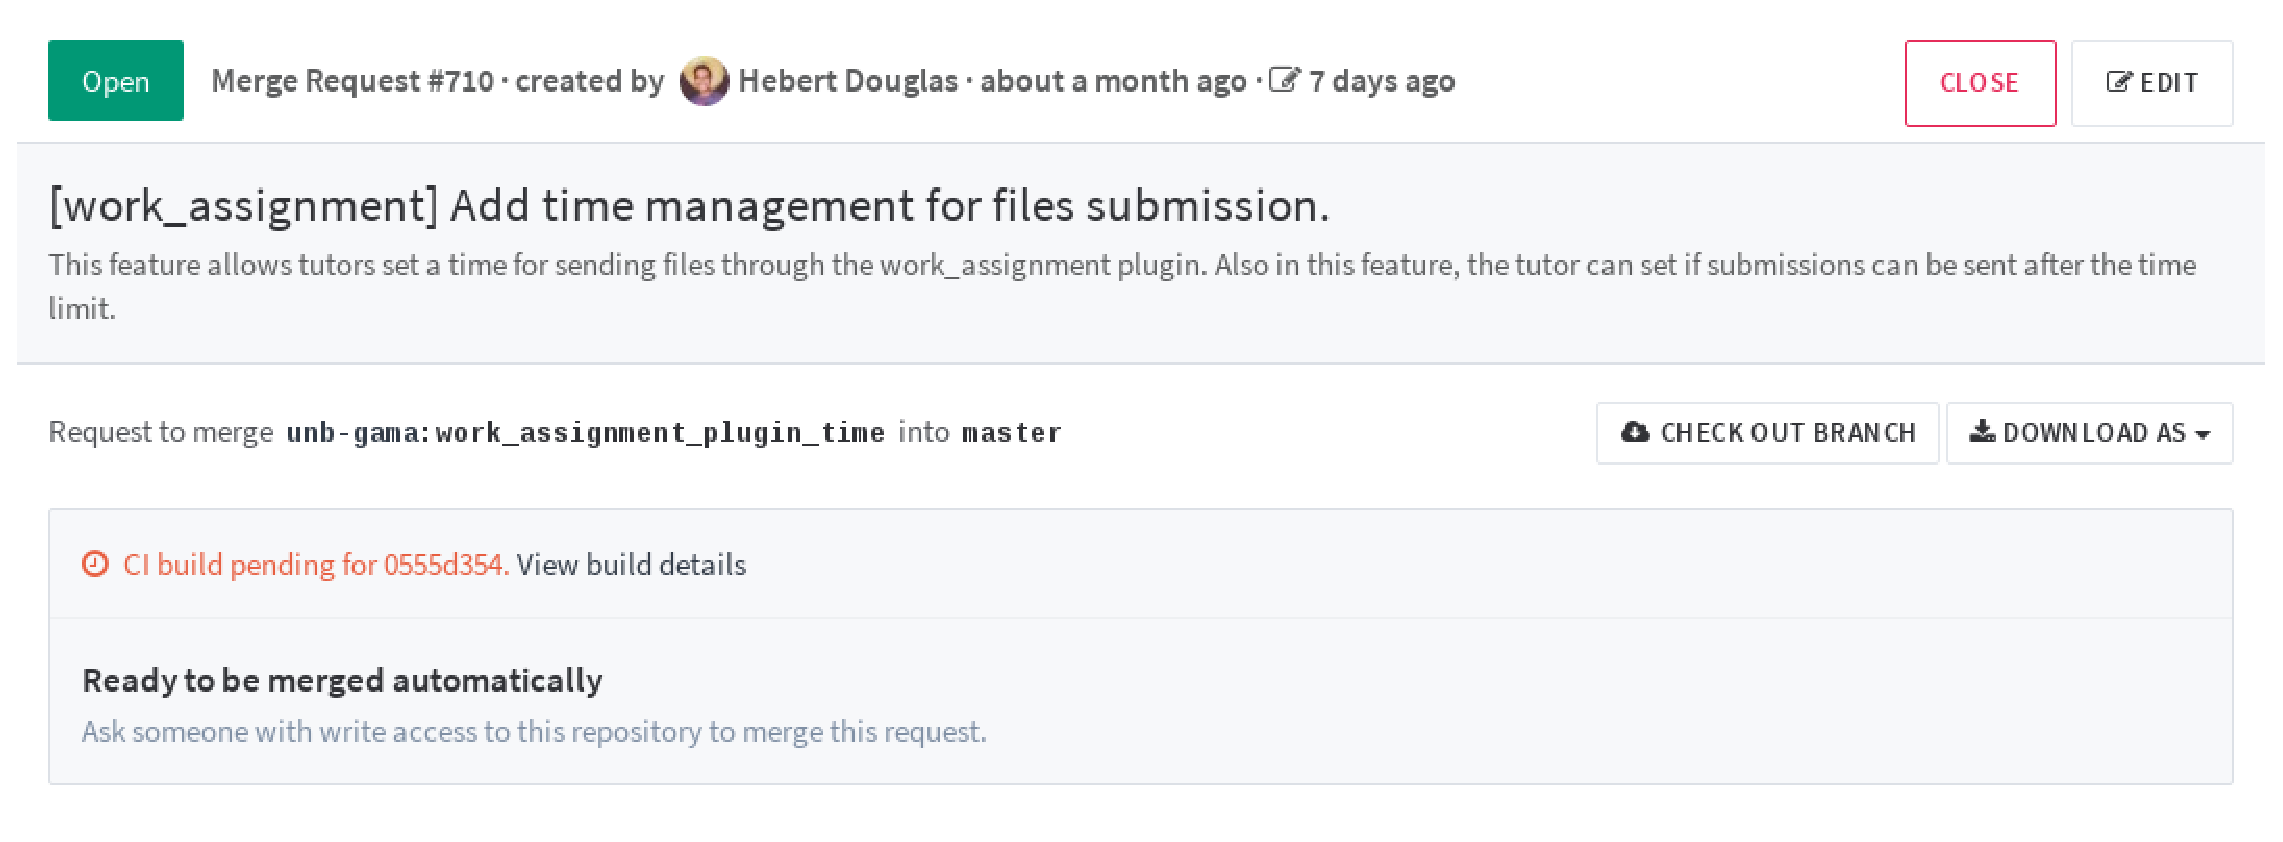
\includegraphics[keepaspectratio=true,scale=0.42]
      {figuras/merge-request710.eps}
    \caption{Merge Request: Gerenciamento de tempo para work\_assignment}
    \label{fig:merge-710}
\end{figure}

A implementação foi revisada por um dos integrantes do Lappis que sugeriu algumas melhorias pontuais, que foram resolvidas durante a revisão. Posteriormente foi realizado o \textit{Merge Request} para a integração do código a \textit{branch \textbf{master}} do Noosfero. Criou-se o Merge Request de número 710\footnote{Disponível em: \url{https://gitlab.com/noosfero/noosfero/merge_requests/710}} (Figura \ref{fig:merge-710}) que ficou em aberto para a revisão dos commiters oficiais da Comunidade. Após alguns dias o mesmo foi revisado pelos desenvolvedores do core do Noosfero, que ainda não alterou o \textit{status} para fechado, mas aprovou a funcionalidade e indicou que se integra ao Noosfero na versão 1\.4.

\begin{figure}[h]
    \centering
    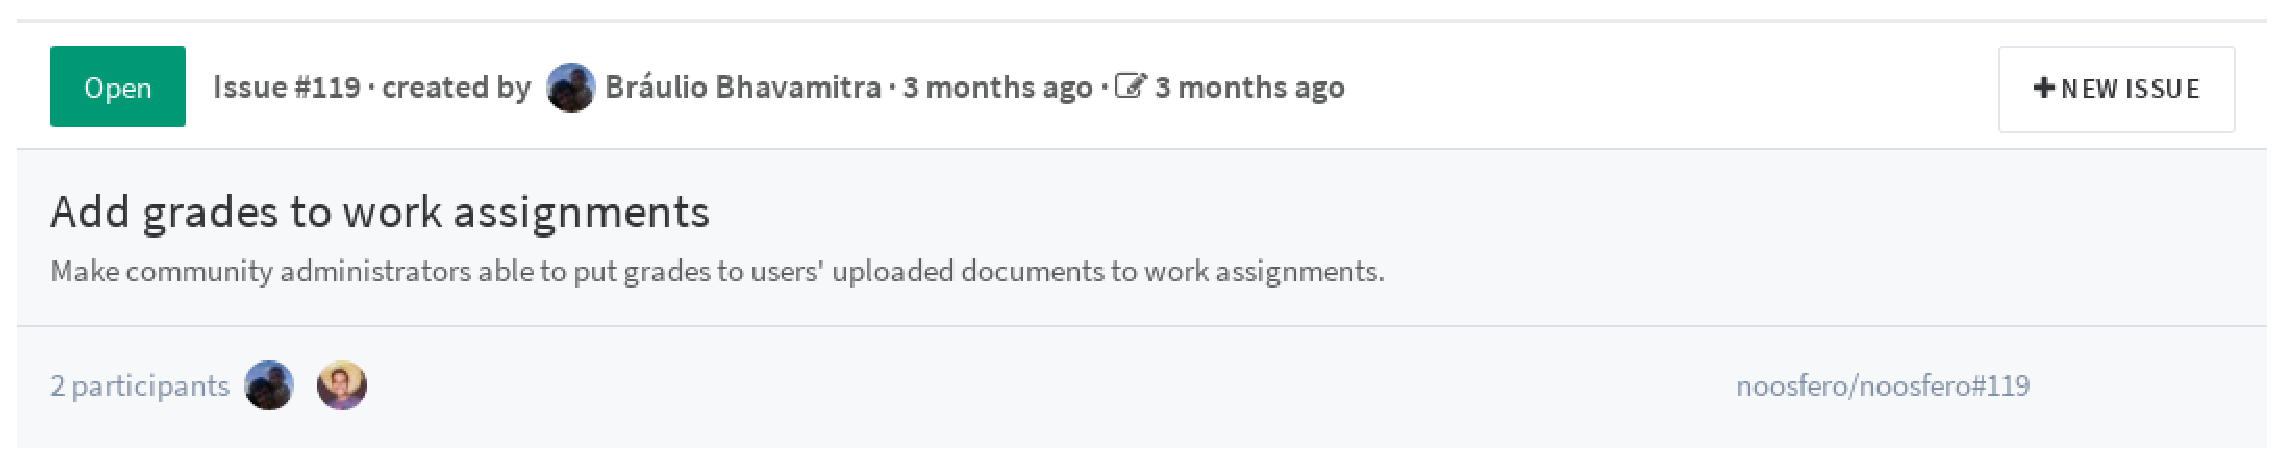
\includegraphics[keepaspectratio=true,scale=0.4]
      {figuras/issue119.eps}
    \caption{Issue 119: Adicionar notas ao \textit{plugin Work Assignment}}
    \label{fig:issue-119}
\end{figure}

Foi iniciada a terceira sprint que engloba a história (\ref{us03}) de ``Atribuir notas aos alunos''. No início da implementação verificou-se que esta funcionalidade já havia sido mapeada por integrante do Noosfero na Issue 119 \footnote{Disponível em: \url{https://gitlab.com/noosfero/noosfero/issues/119}} (Figura \ref{fig:issue-119}), o que favoreceu o desenvolvimento, pois as idéias poderiam ser discutidas evidenciando que o desenvolvimento na comunidade é feito de maneira colaborativa.

No início da terceira \textit{sprint} foram discutidas questões técnicas e arquiteturais de como seria a implementação. A principal discussão foi como seria a realizada a pontuação, por versões ou por pasta, e como seria estabelecida a nota final do aluno. Ficou definido que todas as versões de arquivos enviados poderiam ser pontuados pelos administradores da comunidade e que em uma próxima \textit{sprint} teriam que ser estabelecidos critérios para julgar qual a nota final do aluno.

Na quarta \textit{sprint} foi dado prosseguimento ao desenvolvimento da \ref{us03} onde foi implementado o cenário de uso que proporciona ao administrador definir qual o critério utilizado para a nota final de cada atividade.  Além disso na quarta \textit{sprint} foi implementada a história (\ref{us04}) ``Publicar notas aos alunos'', que permite ao administrador publicar ou omitir notas aos alunos. As funcionalidades desenvolvidas até a quarta \textit{sprint}, englobam requisitos importantes de um AVA, como visto na Seção \ref{ava}.

Apesar da implementação das funcionalidades desenvolvidas, até então não era possível a visualização das notas pelo aluno. Assim sendo, na quinta \textit{sprint} foi implementado a história (\ref{us05}) ``Visualização das notas'', mas foi implementado apenas a tela de visualização da tarefa enviada para permitir a avaliação dos membros da equipe.

Na mesma \textit{sprint} foi implementada a história (\ref{us06}) ``Professor gerencia notas'',que permite ao professor definir módulos que agrupem as atividades a serem enviadas. O objetivo principal é permitir ao administrador modularizar essas atividades. Nessa história não foi implementado o cenário ``Visualizar notas de todos ao alunos de um grupo de atividades'' porque exige uma grande quantidade de requisições ao banco de dados e não traria tanto valor ao usuário.

Como dívida técnica da quinta \textit{sprint}, na sexta \textit{sprint} foi implementada o cenário de uso ``Visualizar notas de todos os alunos de uma determinada atividade'' da \ref{us06}. A idéia principal é disponibilizar de maneira centralizada ao usuário uma forma de visualização das notas de todas atividades, agrupadas pelo seus módulos, para todas as comunidades no qual ele é um membro.

Na sétima \textit{sprint} foi implementada a história (\ref{us07}) ``Blocos de notas recentes'', que visa a criação de um bloco e exibe ao usuário as cinco notas recentes. Devido as sugestões de membros da comunidade deu-se prosseguimento a evolução das telas e padronização das mesmas.

Para oitava \textit{sprint} foi sugerido a criação de um bloco para visualização de todos grupos e suas respectivas atividades. Esta funcionalidade está listada na \ref{us08} (``Bloco para visualização dos módulos'') e foi implementada em paralelo com os testes da história anterior.

Finalizada a execução dessas \textit{sprints}, assim como realizado na primeira issue foi realizado o \textit{Merge Request} para a integração do código a \textit{branch \textbf{master}} do Noosfero. Criou-se o Merge Request de número XXX\footnote{Disponível em: \url{https://gitlab.com/noosfero/noosfero/merge_requests/XXX}} (Figura \ref{fig:merge-XXX}) que ficou em aberto para a revisão dos \textit{commiters} oficiais da Comunidade.

Na nona e última \textit{sprint} foi criado um ambiente de homologação para o Comunidade.UnB afim de testar as novas funcionalidades e a autenticação com o LDAP. Para validar o novo mecanismo de autenticação o CPD da FGA forneceu acesso a base de dados do seu servidor LDAP, a mesma utilizada para o controle de acesso a rede \textit{wireless} do campus, e durante os testes no servidor de homologação a funcionalidade teve o comportamento esperado.

Nesse processo de desenvolvimento fica evidente a aplicação das práticas adotadas pela comunidade de software livre Noosfero. Foi executado o processo desde a criação de uma \textit{Issue}, passando por todo o processo de desenvolvimento adotando práticas ágeis, até o encerramento desse ciclo com a criação do \textit{Merge request}. Vale lembrar que mesmo após a revisão e integração ao \textit{core} o código ainda se encontra em constante evolução.

% -------------------- Evolução do Work Assignment ----------------
\section{Evolução do \textit{plugin Work Assignment}}

Nesta seção serão apresentadas os resultados correspondentes a evolução do \textit{plugin Work Assignment}, que até então detinha apenas a funcionalidade para permitir o envio de arquivos para o servidor em um determinado período de tempo.

A proposta de evolução é a criação de um sistema de notas que permita ao professor atribuir notas as atividades enviadas e dessa maneira acompanhar a situação de cada aluno. Do ponto de vista do aluno, o mesmo poderá visualizar todas as notas das atividades em cada disciplina, avaliando se o seu desempenho está satisfatório.

A partir das evoluções realizada no plugin work assignmnet permitem que o administrador de uma comunidade (professor), realize a modularização das atividades a serem entregues, o que facilita a ele a organização do curso e possibilita uma melhor visualização dos alunos.

Ao definir um módulo para seu curso, o professor informa a data de início e fim para o mesmo, e dessa maneira todas as atividades que farão parte desse módulo deve estar entre o período determinado.

\begin{figure}[h]
    \centering
    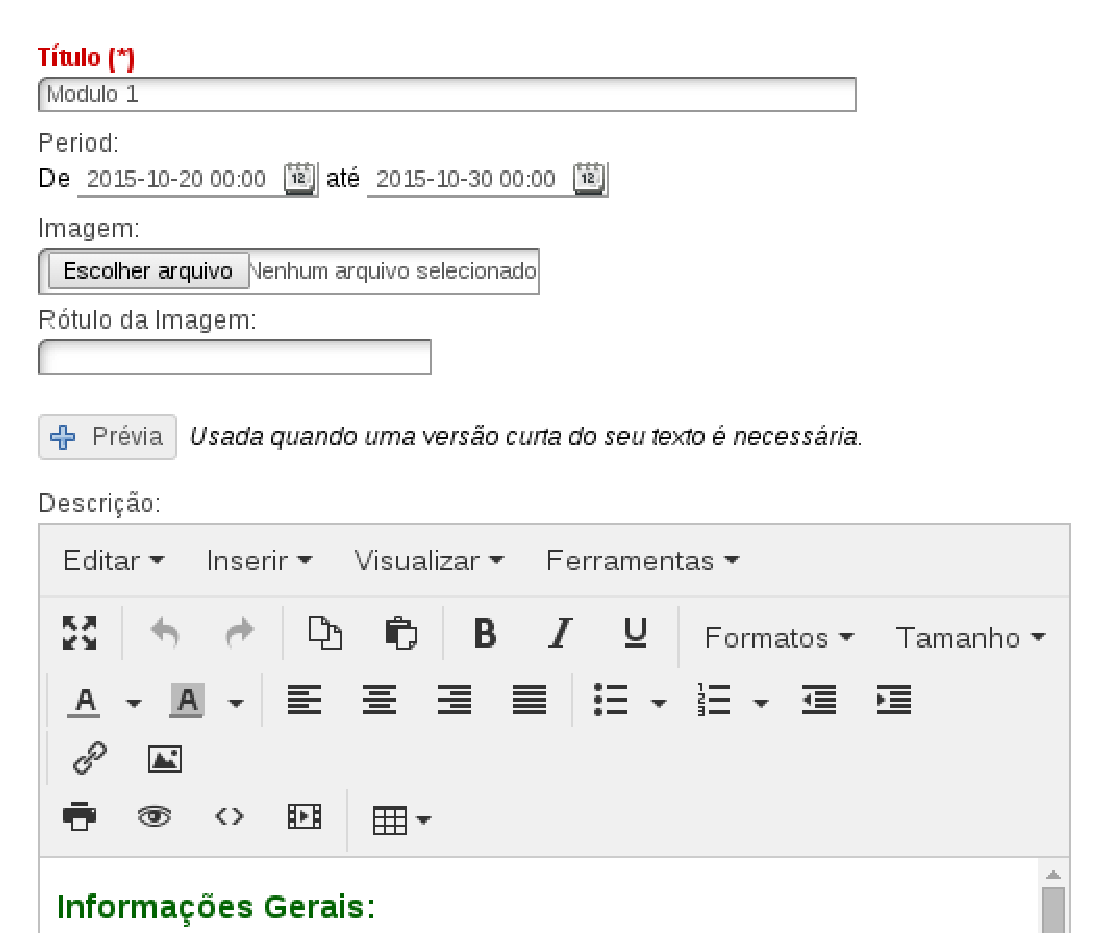
\includegraphics[keepaspectratio=true,scale=0.6]
      {figuras/work-assignment-group.eps}
    \caption{Tela para criação de grupos de trabalhos a serem enviados.}
    \label{fig:work-assignment-group}
\end{figure}

Para criar um módulo o administrador agora pode entrar no painel de controle da comunidade e adicionar um novo tipo de conteúdo denominado como ``Grupo de Trabalhos a serem enviados''. Dentro desse conteúdo o usuário deve informar o título, período, uma prévia do que será aquele módulo e sua descrição detalhada, conforme pode ser visualizado na Figura \ref{fig:work-assignment-group}.

\begin{figure}[h]
    \centering
    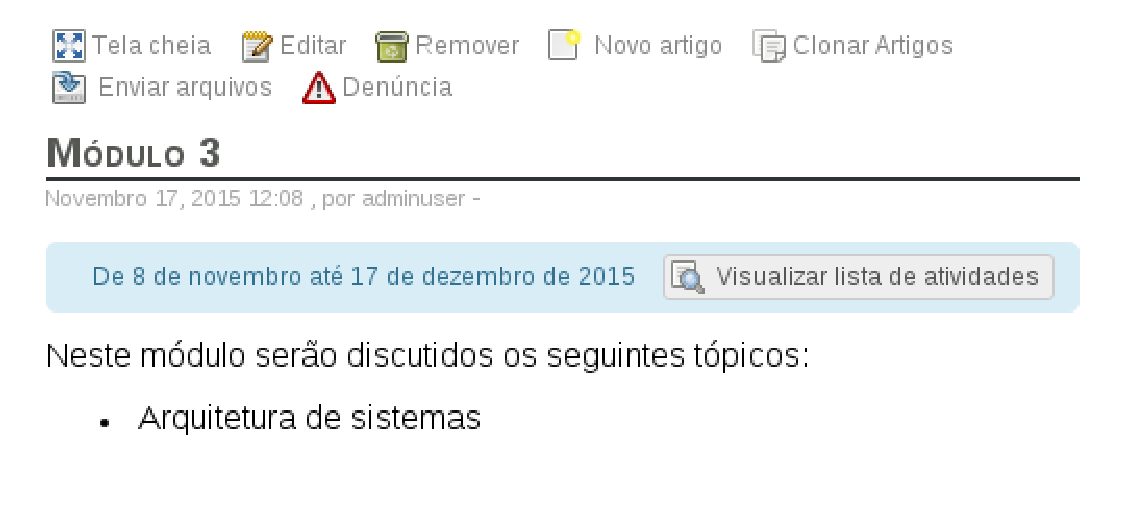
\includegraphics[keepaspectratio=true,scale=0.6]
      {figuras/principal-group.eps}
    \caption{Tela principal de um módulo.}
    \label{fig:principal-group}
\end{figure}

Após salvar esse grupo de trabalho o usuário é redirecionado para o módulo criado. Nesta tela é exibido ao usuário a descrição e o período referente ao módulo, existe ainda um botão denominado como ``Visualizar lista de atividades'', que mostra ao usuário ou administrador a lista de todas as atividades daquele módulo. Como pode ser visualizado na Figura \ref{fig:principal-group}.

\begin{figure}[h]
    \centering
    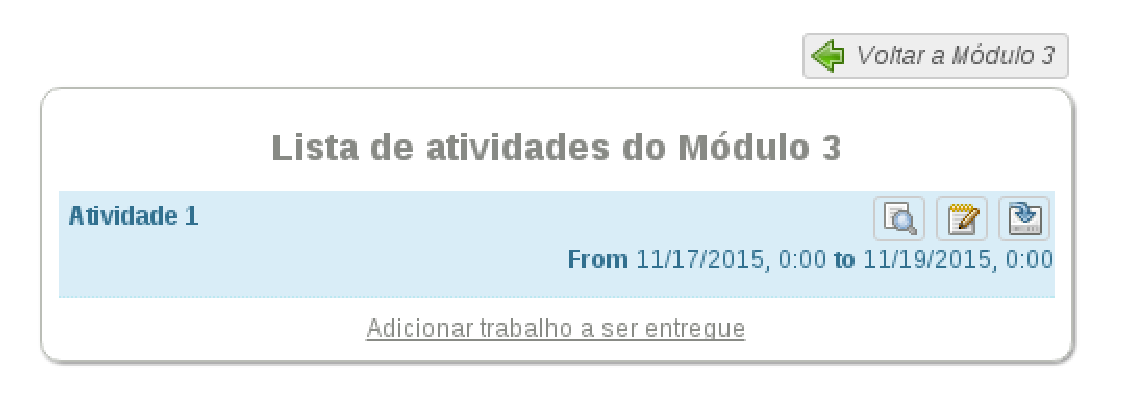
\includegraphics[keepaspectratio=true,scale=0.6]
      {figuras/lista-atividades.eps}
    \caption{Lista de atividades de um \textit{work assignment}.}
    \label{fig:lista-atividades}
\end{figure}

Na Figura \ref{fig:lista-atividades} é exbido a lista de atividades referentes ao módulo criado, nesse caso com apenas uma atividade, também é disponibilizado ao usuário um \textit{link} (``Adicionar trabalho a ser entregue'') que redireciona o usuário para a página principal de criação de trabalhos.

\begin{figure}[h]
    \centering
    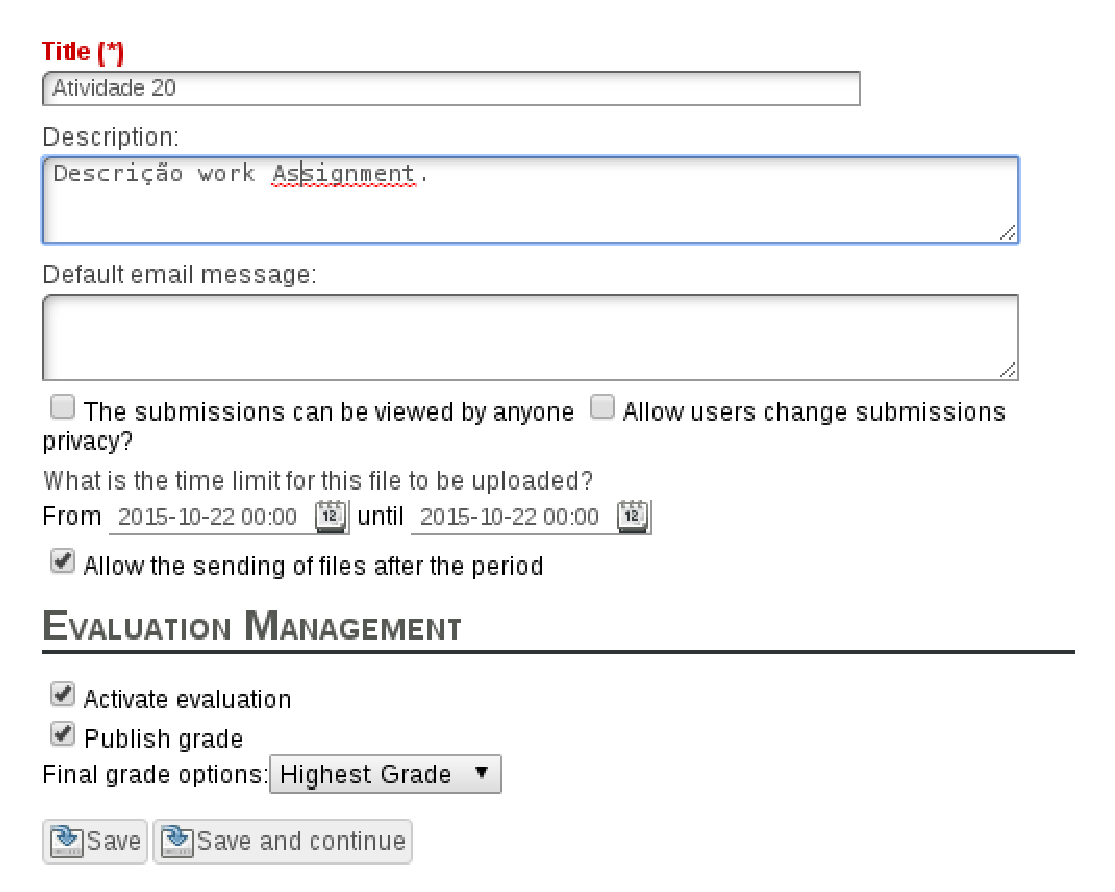
\includegraphics[keepaspectratio=true,scale=0.6]
      {figuras/work-assignment-final.eps}
    \caption{Tela para criação de um \textit{work assignment}.}
    \label{fig:work-assignment-final}
\end{figure}

Dentro desse conteúdo é solicitado ao usuário informações básicas sobre o trabalho, além disso é definido o período que a atividade ficará em aberto e se é possível o envio após a data limite. Na mesma tela temos o gerenciamento das avaliações que permite ativar o modo de avaliação e publicar as notas de acordo com o critério de avaliação. Na Figura \ref{fig:work-assignment-final} é possível verificar como está a tela de criação de um novo ``Trabalho a ser entregue''.

\begin{figure}[h]
    \centering
    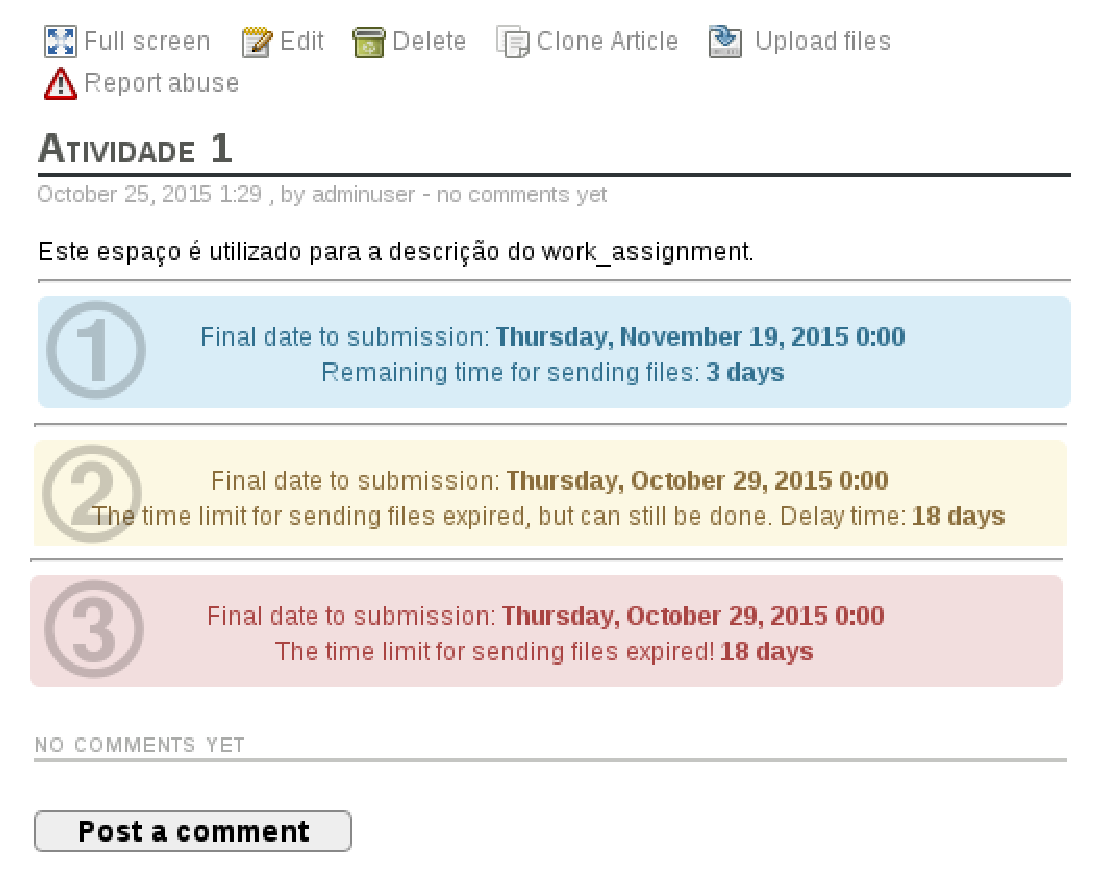
\includegraphics[keepaspectratio=true,scale=0.6]
      {figuras/work-status.eps}
    \caption{Representação do estado dos trabalhos a serem entregues.}
    \label{fig:work-status}
\end{figure}

Como citado, uma das opções deste conteúdo é informar qual é o tempo limite para que o envio de arquivos. Buscando a melhor forma de visualização para os usuários foram criados modos de visualização e para isso definiu-se três estados de envio:

\begin{itemize}
\item Aberto: exibe o tempo definido para aquela atividade e o tempo ainda restante para o término do envio (Figura \ref{fig:work-status}, item 1)
\item Permitido: o usuário é informado se o período de envio já expirou e quanto tempo já se passou após a data limite (Figura \ref{fig:work-status}, item 2)
\item Expirado: exibe o tempo definido para a atividade e que a mesma está expirada. (Figura \ref{fig:work-status}, item 3)
\end{itemize}

Para que o usuário visualize a atividade e saiba de imediato em qual situação ela se encontra, foi utilizado um esquema de cores que fica como plano de fundo do tempo ainda restante. De acordo com a figura \ref{fig:work-status} podemos visuzalizar que foram utilizadas três cores: o verde para representar que a atividade está em aberto (Item 1), o laranja para informar que é permitido (Item 2), e o vermelho para indicar que está fechada (Item 3). É importante ressaltar que a Figura \ref{fig:work-status} exibe os três estados disponíveis, mas para cada ``Trabalho a ser entregue'' é exibido apenas um de acordo com a situação.

\begin{figure}[h]
    \centering
    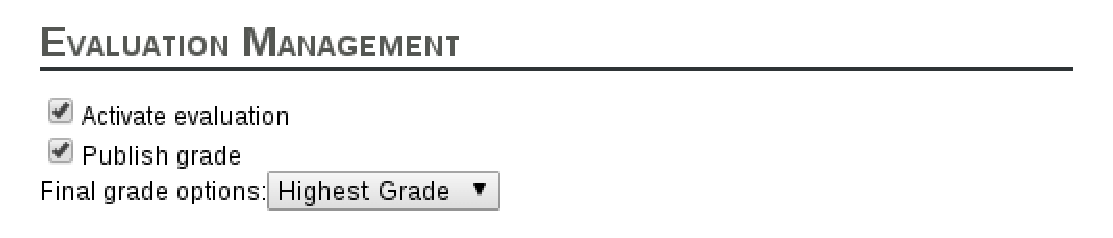
\includegraphics[keepaspectratio=true,scale=0.75]
      {figuras/evaluation-management.eps}
    \caption{Tela para o gerenciamento de avaliações.}
    \label{fig:evaluation-management}
\end{figure}

Ainda na tela para de criação de trabalhos a serem enviados, é relevante analisar as funcionalidades do gerencimento de avaliações. É importante ressaltar que para cada ``Trabalho a ser enviado'' o administrador pode escolher se deseja ou não publicar as notas para os alunos, permitindo ao mesmo realizar todas as avaliações antes de publicá-las.

O gerenciamento também proporciona ao administrador definir qual o critério utilizado para a nota final de cada atividade. Foram determinados três critérios:
\begin{itemize}
\item Maior nota: é exibida como nota final a maior nota de todas as versões pontuadas.
\item Mais Recente: é exibida como nota final a última versão pontuada.
\item Nota opcional: no momento da avalição de cada versão o administrador define qual é a nota final
\end{itemize}

Essas funcionalidades permitem flexibilidade quanto ao critério de avaliação do professor e trazem maior liberdade para realizar as avalições. A opções do gerenciamento de notas estão evidenciadas na Figura \ref{fig:evaluation-management}.

Caso o professor tenha habilitado a opção de ``Ativar Avaliação'' esteja ativada o professor pode pontuar os arquivos enviados pelos usuários. Como o \textit{plugin} permite o envio de mais de uma versão para a mesma atividade, foi definido que todas elas poderiam ser pontuados e a nota final é dada de acordo com os critérios estabelecidos.

\begin{figure}[h]
    \centering
    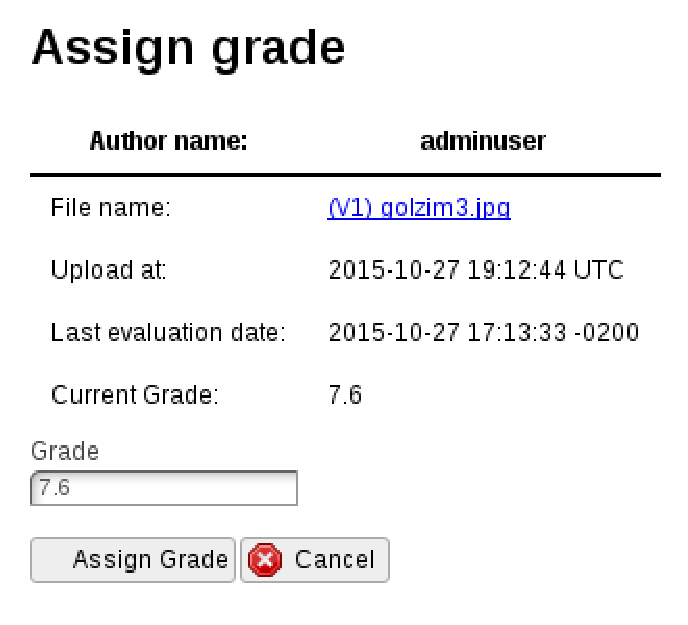
\includegraphics[keepaspectratio=true,scale=0.6]
      {figuras/assign-grade.eps}
    \caption{Tela para atribuição e alteração da notas.}
    \label{fig:assign-grade}
\end{figure}

A partir disso, na visualização da lista de trabalhos enviados o professor pode selecionar a opção ``atribuir nota'' que o redireciona para a tela que permite atribuir e alterar a nota de cada arquivo enviado, conforme evidenciado na Figura \ref{fig:assign-grade}.

Essa tela exibe ao usuário informações relevantes no momento da avaliação como o nome do arquivo a ser avaliado, a data de envio, a data da última avaliação e, caso haja, a nota atual daquele arquivo. Além disso está disposto um campo que permite atribuir a nova nota ao aluno.

\begin{figure}[h]
    \centering
    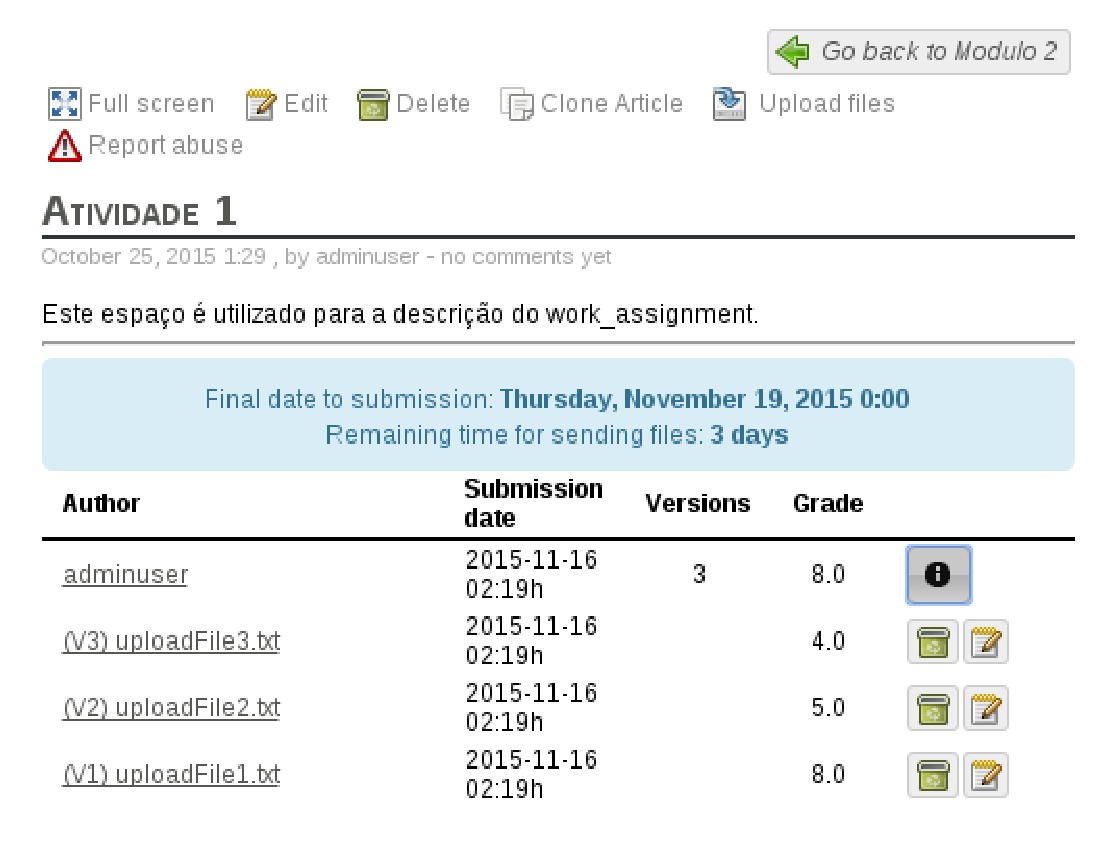
\includegraphics[keepaspectratio=true,scale=0.6]
      {figuras/visualiza-notas.eps}
    \caption{Visualização das notas de trabalhos enviados.}
    \label{fig:visualiza-notas}
\end{figure}

Desde que a avaliação esteja ativa e o administrador tenha permitido a visualização das notas, é criada uma coluna que é exibe a nota final do aluno e a pontuação de cada versão avaliada. Este comportamento é evidenciado na Figura \ref{fig:visualiza-notas}.

Apesar da disponibilização das notas, ainda era necessário que o usuario procura-se cada uma das atividades para visualização das notas. Foi implementado uma funcionalidade que tem como principal obejtivo centralizar todas atividades de um usuário e deste modo organizá-las dentro de seus módulos e as comunidades pertencentes.

\begin{figure}[h]
    \centering
    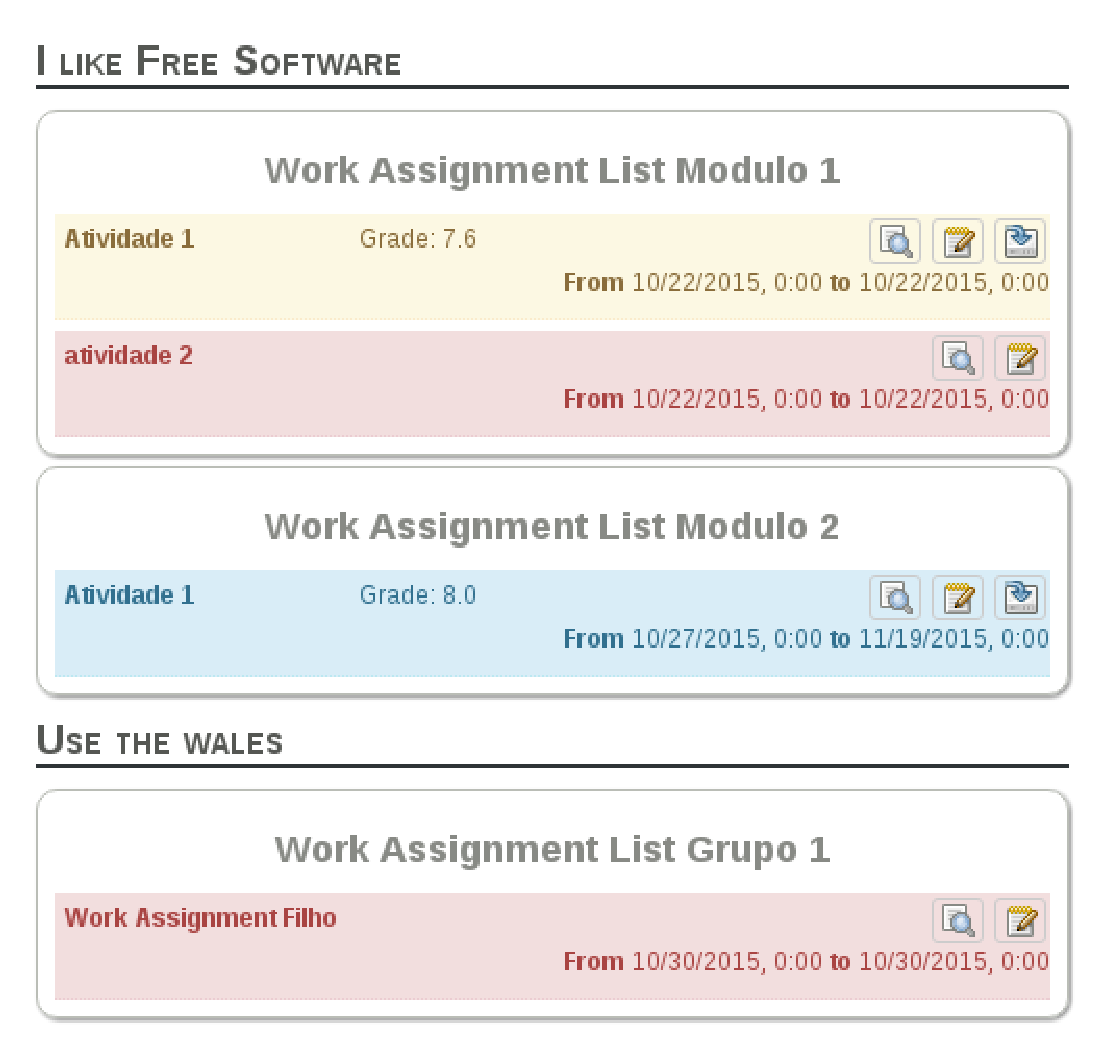
\includegraphics[keepaspectratio=true,scale=0.5]
      {figuras/work-assignment-group-list.eps}
    \caption{Tela para visualização das atividades de forma centralizada.}
    \label{fig:group-list}
\end{figure}

No painel de controle de cada usuário foi criado uma nova funcionalidade chamada de ``Meus Cursos'' que ao ser clicada redireciona o usuário a uma lista de todas as comunidades no qual é membro e utilizam que possuem algum tipo de conteúdo relacionado ao grupo de atividades. Conforme evidenciado na Figura \ref{fig:group-list}, é exibido todas as atidades em seus respectivos grupos.

Utilizando a personalização que o Noosfero oferece, foram criados blocos que permitem ao usuário flexibilidade quanto ao posicionamento e exibição do mesmo. Esses blocos beneficiam o usuário quanto ao \textit{feedback} sobre suas notas. Conforme pode ser visualizado a esquerda na Figura \ref{fig:blocos}, esse bloco exibe ao usuário as cinco notas mais recentes.

\begin{figure}[h]
    \centering
    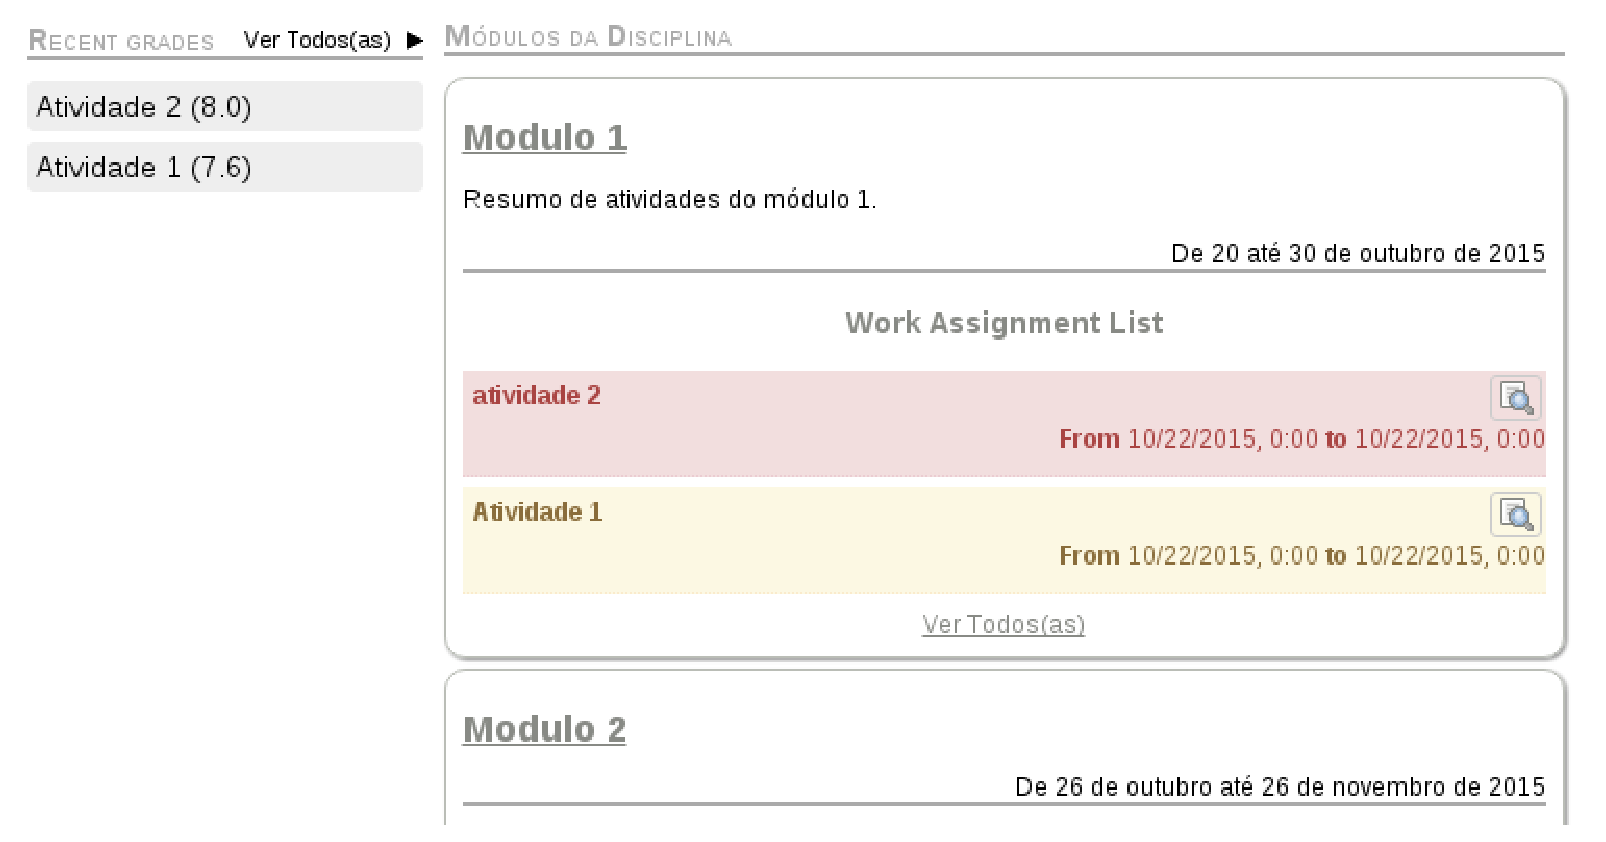
\includegraphics[keepaspectratio=true,scale=0.5]
      {figuras/blocos.eps}
    \caption{Blocos para visualização das atividades.}
    \label{fig:blocos}
\end{figure}


Na Figura \ref{fig:blocos} evidencia-se o bloco para visualização de todos grupos e suas respectivas atividades. Por padrão são exibidas apenas três atividades por grupo, mas é permitido ao administrador da comunidade escolher quantas deseja.

No contexto da UnB, o desenvolvimento a funcionalidades deenvolvidas são importantes, pois segundo o documento da instituição \citeonline[p. 37]{unb-professor}, as notas para os alunos auxiliam a assimilação progressiva de conhecimento, e sabe-se que permite um maior \textit{feedback} para o aluno, pois nem sempre fica transparente o seu desempenho ao longo do semestre.

Em resumo, as funcionalidades apresentadas neste capítulo colaboram para uso do Comunidade.UnB, tornando-o uma plataforma híbrida entre um ambiente virtual de aprendizagem e uma rede social, para a troca de conhecimento através das comunidades e perfis de usuários. Assim, permitindo englobar departamentos, organizações e projetos específicos da Universidade de Brasília.

\subsection{Arquitetura do Plugin Work Assignment}

Sabendo que o Noosfero está em constante evolução o \textit{plugin work assignment} passará por melhorias durante sua vida útil. Sabendo disso é importante entender como se onfigura a sua arquitetura após as implementações realizadas, afim de compreender quais as classes compõe sua estrutura e como se relacionam.

\begin{figure}[h]
    \centering
    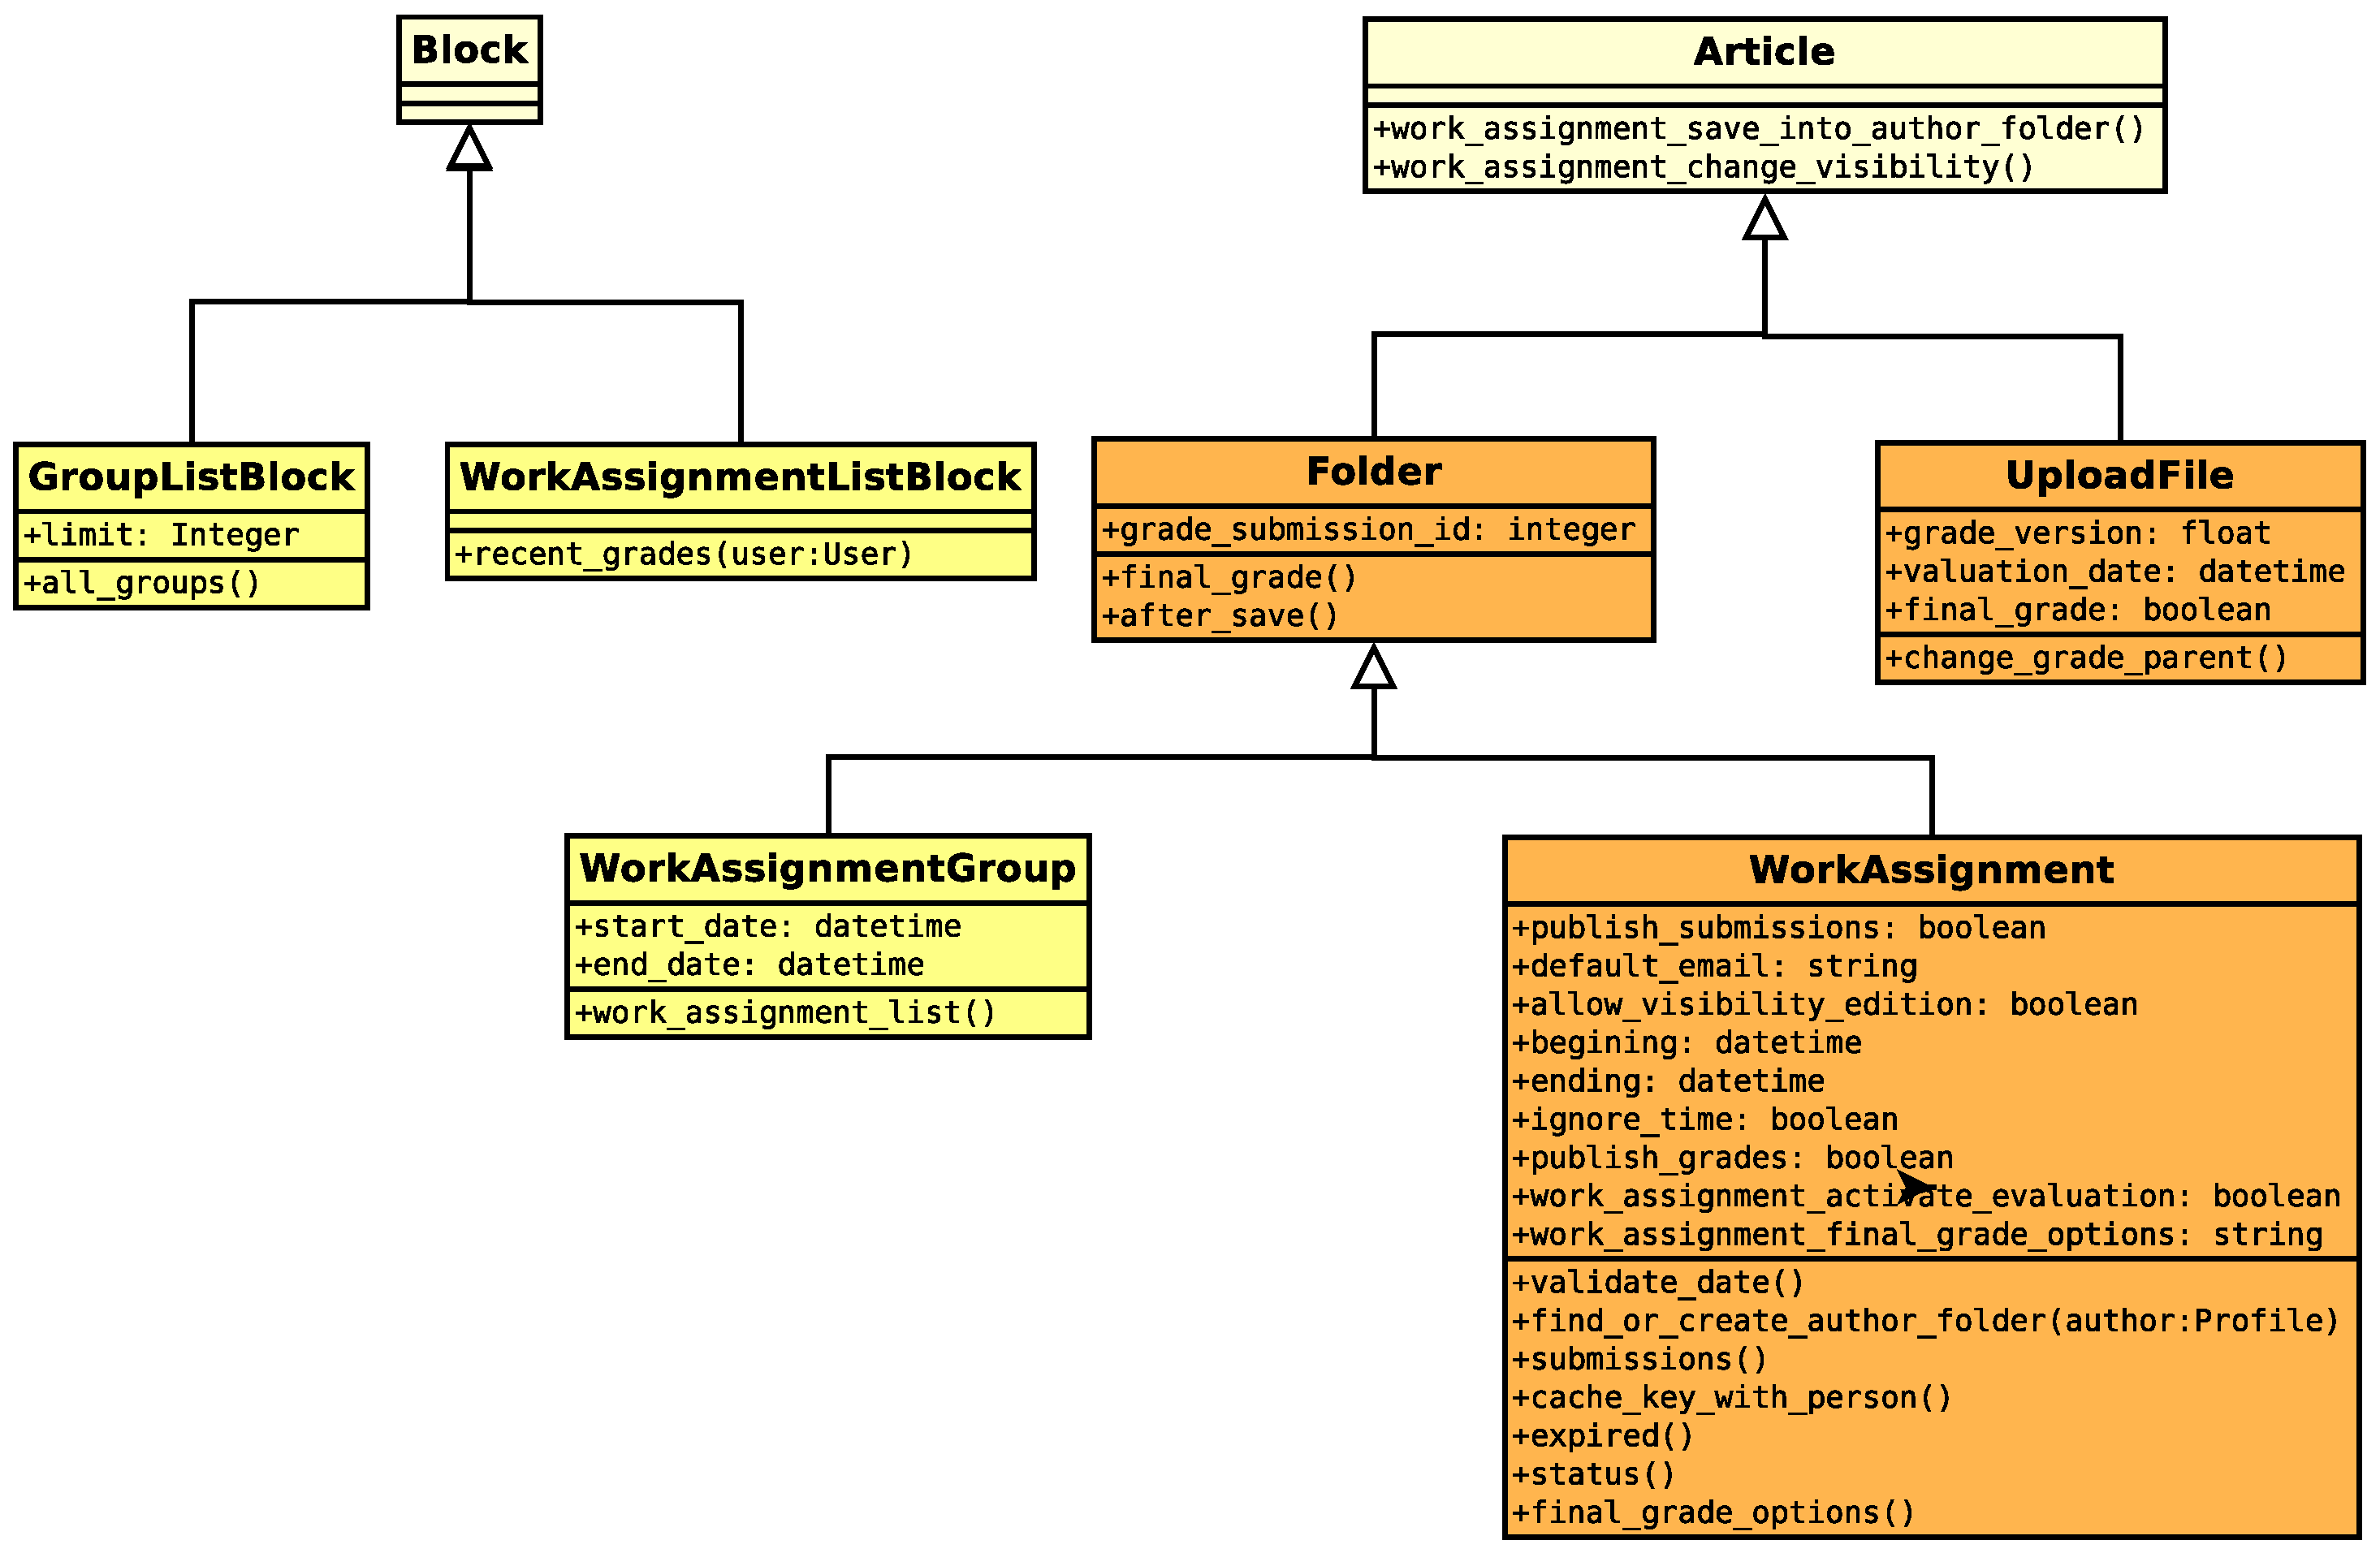
\includegraphics[keepaspectratio=true,scale=0.3]
      {figuras/diagramaUMLCompletoColor.eps}
    \caption{Diagrama de classes do \textit{Plugin Work Assignment}}
    \label{fig:arquitetura-work}
\end{figure}

A Figura \ref{fig:arquitetura-work} evidencia as principais classes utilizadas pelo \textit{plugin}, no qual foram criadas as classes \textit{GroupListBlock, WorkAssignmentListBLock, WorkAssignmentGroup}, e apenas modificadas as \textit{WorkAssignment, UploadFile, Folder} e \textit{Article, Block} que não sofreram modificações durante este processo de evolução.

No desenvolivmento foi criado uma especialização da classe \textit{Folder} denominada como \textit{WorkAssignmentGroup}, que possibilita ao administrador criar pastas que representam grupos de atividades e tem como principal caracterísitca data de início e fim.

No funcionamento do \textit{plugin}, quando um usuário cria um ``Grupo de Atividades'' é possível inserir qualquer tipo de \textit{Article} dentro dessa pasta, dessa maneira é possível criar um ``Trabalho a ser enviado'' (\textit{WorkAssignment}). A partir disso os membros da comunidade podem enviar seus arquivos como resposta a atividade, e quando o envio é realizado o \textit{plugin} cria uma pasta (\textit{Folder}) para cada usuário e a associa ao arquivo enviado (\textit{UploadFile}). 

Na solução foi levado em consideração que todos os arquivos enviados por uma única pessoa poderiam ser pontuados, deixando de forma opcional qual seria o critério para a nota final. Para isso foram criados dois atributos (grade\_version, valuation\_date) na classe \textit{UploadFile}, que armazenam a nota da versão enviada e a data da avaliação, assim uma vez que a pontuação de uma versão é alterada a nota final do aluno se modifica de acordo com o critério de avaliação.

As classes \textit{WorkAssignmentListBlock} e \textit{GroupListBlock} são uma especialização de \textit{Block} responsáveis por disponibilizar ao usuário a opção de blocos que exibem as notas recentes e listam todos os grupos de uma comunidade, respectivamente.

Entendendo esse funcionamento verifica-se que a arquitetura tornou o \textit{plugin} flexível ao ponto que todas essas classe principais (\textit{WorkAssignmentGroup, WorkAssignment, UploadFile, Folder}) podem ser criadas independente umas das outras. A dependência está relacionada aos blocos que são dispensáveis caso não exista trabalhos a serem enviados ou grupos de atividades.

% Teams Work_assignment https://gitlab.com/noosfero/noosfero/issues/134

% Com o objetivo de permitir ao administrador realizar uma modularização das atividades, foi criada uma nova classe \textit{WorkAssignmentPlugin::WorkAssignmentGroup}, que representa um grupo de atividades e tem como funcionalidade básica definir um período para o mesmo.

\section{Evolução do \textit{plugin Comunidade.UnB}}
\label{plugin-comunidade}

O objetivo do \textit{plugin} do Comunidade.Unb é que o usuário tenha acesso através dos mesmos dados utilizados para acessar outros serviços, como, por exemplo, o serviço de matrícula \footnote{Disponível em: \url{https://matriculaweb.unb.br}} para alunos ou o serviço de lançamento de notas para professores.

A versão anterior do \textit{plugin} permitia que apenas os novos usuários realizassem o cadastro de suas matrículas, dessa maneira aqueles que já estavam cadastrados não tinham acesso ao portal. Devido às limitações de acesso definidas pelo \textit{plugin}, onde apenas usuários com matrícula cadastrada tem acesso ao sistema.

Foi criada nova versão do \textit{plugin} que permite cadastrar a matrícula dos usuários que já possuem registro no Comunidade.UnB. Dessa maneira, o \textit{plugin Comunidade.UnB} é ativado permitindo a autenticação apenas dos usuários cadastrados no LDAP da universidade. Esta base de dados contempla alunos, professores, servidores técnico-administrativos que queiram utilizar a rede. A história de usuário (\ref{us09}) com seus respectivos cenários de uso, encontram-se disponíveis no Apêndice \ref{apen-historia-usuario}.

\begin{figure}[h]
    \centering
    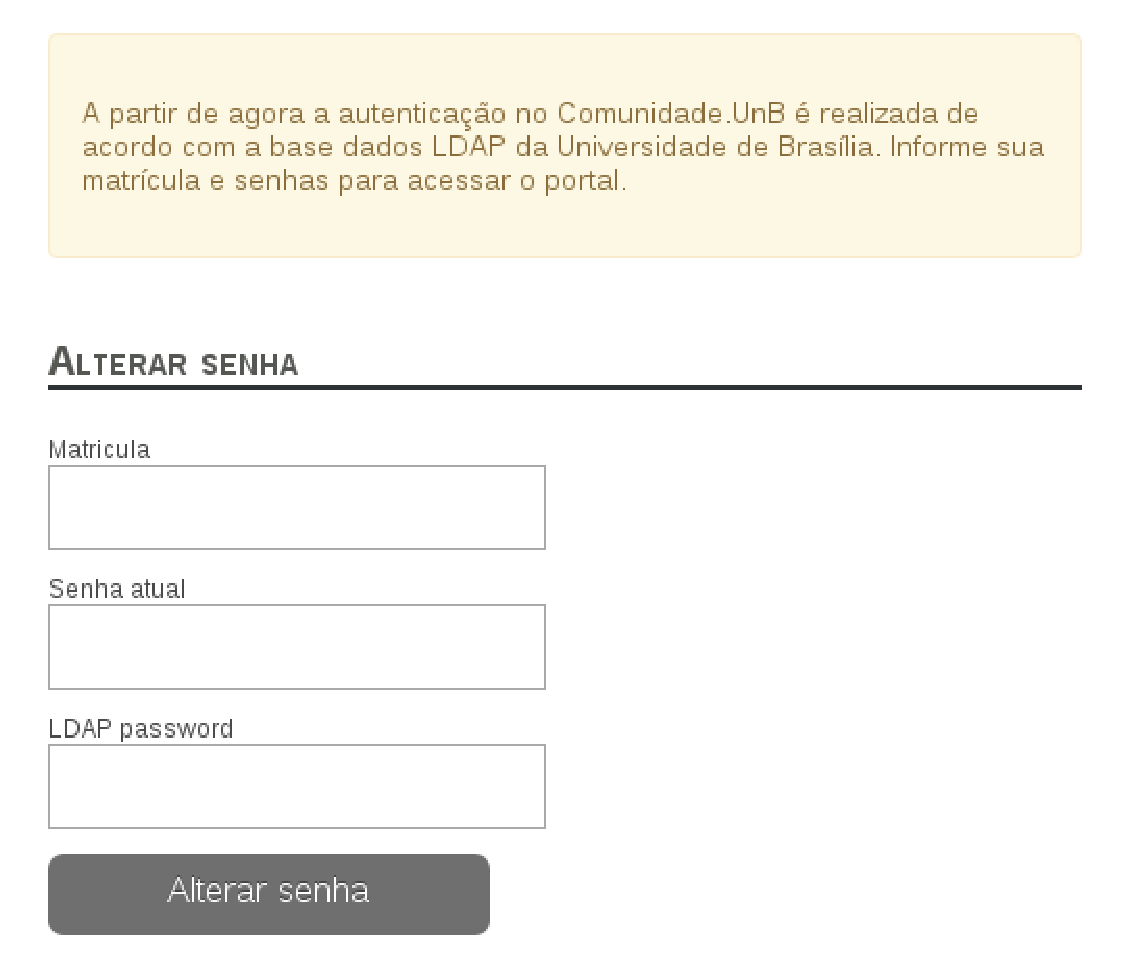
\includegraphics[keepaspectratio=true,scale=0.5]
      {figuras/associate-matricula.eps}
    \caption{Tela para assoicar matricula ao usuário.}
    \label{fig:associate-matricula}
\end{figure}

Com a nova funcionaliadade após o usuário realizar o Login, ele é redirecionado para uma tela que solicita a matrícula e senhas, a utilizada para logar no Portal e a do LDAP, conforme a Figura \ref{fig:associate-matricula}. O sistema verifica os dados na base de dados LDAP e caso seja confirmado, cadastra matrícula e altera a senha do usuário.

Foi retirado a funcionalidade de alteração e recuperação de senha uma vez que queremos manter a compatibilidade entre a rede Comunidade.UnB e os demais serviços. Desta forma, caso o usuário deseje trocar sua senha, o mesmo deve procurar o CPD e solicitar a alteração.

Com o objetivo de utilizar este \textit{plugin} em um ambiente de produção é necessário solicitar acesso ao LDAP de alunos do matricula web, visto que o da FGA segue um mesmo padrão de senha para todos os usuários, dessa forma todos ficariam com suas contas vulneráveis à acessos indevidos.

Como visto o \textit{plugin} traz para o Comunidade.UnB maior controle sobre seus usuários, centralizando o acesso para o escopo da Universidade.
